% Options for packages loaded elsewhere
\PassOptionsToPackage{unicode}{hyperref}
\PassOptionsToPackage{hyphens}{url}
%
\documentclass[
]{article}
\usepackage{amsmath,amssymb}
\usepackage{lmodern}
\usepackage{ifxetex,ifluatex}
\ifnum 0\ifxetex 1\fi\ifluatex 1\fi=0 % if pdftex
  \usepackage[T1]{fontenc}
  \usepackage[utf8]{inputenc}
  \usepackage{textcomp} % provide euro and other symbols
\else % if luatex or xetex
  \usepackage{unicode-math}
  \defaultfontfeatures{Scale=MatchLowercase}
  \defaultfontfeatures[\rmfamily]{Ligatures=TeX,Scale=1}
\fi
% Use upquote if available, for straight quotes in verbatim environments
\IfFileExists{upquote.sty}{\usepackage{upquote}}{}
\IfFileExists{microtype.sty}{% use microtype if available
  \usepackage[]{microtype}
  \UseMicrotypeSet[protrusion]{basicmath} % disable protrusion for tt fonts
}{}
\usepackage{xcolor}
\IfFileExists{xurl.sty}{\usepackage{xurl}}{} % add URL line breaks if available
\IfFileExists{bookmark.sty}{\usepackage{bookmark}}{\usepackage{hyperref}}
\hypersetup{
  pdftitle={The Bayesian Inferential Paradigm in Archaeology},
  pdfauthor={ERIK OTÁROLA-CASTILLO*, MELISSA G. TORQUATO; Department of Anthropology, Purdue University, West Lafayette, Indiana, USA; CAITLIN E. BUCK; School of Mathematics and Statistics, University of Sheffield, Sheffield, UK},
  hidelinks,
  pdfcreator={LaTeX via pandoc}}
\urlstyle{same} % disable monospaced font for URLs
\usepackage[margin=1in]{geometry}
\usepackage{longtable,booktabs,array}
\usepackage{calc} % for calculating minipage widths
% Correct order of tables after \paragraph or \subparagraph
\usepackage{etoolbox}
\makeatletter
\patchcmd\longtable{\par}{\if@noskipsec\mbox{}\fi\par}{}{}
\makeatother
% Allow footnotes in longtable head/foot
\IfFileExists{footnotehyper.sty}{\usepackage{footnotehyper}}{\usepackage{footnote}}
\makesavenoteenv{longtable}
\usepackage{graphicx}
\makeatletter
\def\maxwidth{\ifdim\Gin@nat@width>\linewidth\linewidth\else\Gin@nat@width\fi}
\def\maxheight{\ifdim\Gin@nat@height>\textheight\textheight\else\Gin@nat@height\fi}
\makeatother
% Scale images if necessary, so that they will not overflow the page
% margins by default, and it is still possible to overwrite the defaults
% using explicit options in \includegraphics[width, height, ...]{}
\setkeys{Gin}{width=\maxwidth,height=\maxheight,keepaspectratio}
% Set default figure placement to htbp
\makeatletter
\def\fps@figure{htbp}
\makeatother
\setlength{\emergencystretch}{3em} % prevent overfull lines
\providecommand{\tightlist}{%
  \setlength{\itemsep}{0pt}\setlength{\parskip}{0pt}}
\setcounter{secnumdepth}{-\maxdimen} % remove section numbering
\usepackage{setspace}\doublespacing
\usepackage[labelfont=bf,width=1\textwidth,justification=raggedright,singlelinecheck=false]{caption}
\captionsetup[figure]{labelfont=bf}
\usepackage[pagewise]{lineno}
\ifluatex
  \usepackage{selnolig}  % disable illegal ligatures
\fi
\newlength{\cslhangindent}
\setlength{\cslhangindent}{1.5em}
\newlength{\csllabelwidth}
\setlength{\csllabelwidth}{3em}
\newenvironment{CSLReferences}[2] % #1 hanging-ident, #2 entry spacing
 {% don't indent paragraphs
  \setlength{\parindent}{0pt}
  % turn on hanging indent if param 1 is 1
  \ifodd #1 \everypar{\setlength{\hangindent}{\cslhangindent}}\ignorespaces\fi
  % set entry spacing
  \ifnum #2 > 0
  \setlength{\parskip}{#2\baselineskip}
  \fi
 }%
 {}
\usepackage{calc}
\newcommand{\CSLBlock}[1]{#1\hfill\break}
\newcommand{\CSLLeftMargin}[1]{\parbox[t]{\csllabelwidth}{#1}}
\newcommand{\CSLRightInline}[1]{\parbox[t]{\linewidth - \csllabelwidth}{#1}\break}
\newcommand{\CSLIndent}[1]{\hspace{\cslhangindent}#1}

\title{\textbf{The Bayesian Inferential Paradigm in Archaeology}}
\author{ERIK OTÁROLA-CASTILLO*, MELISSA G. TORQUATO \and Department of
Anthropology, Purdue University, West Lafayette, Indiana,
USA \and CAITLIN E. BUCK \and School of Mathematics and Statistics,
University of Sheffield, Sheffield, UK}
\date{\emph{R Markdown version last compiled on Monday September 20
2021, 21:24:04, UTC}}

\begin{document}
\maketitle

\vspace{4cm}

\noindent \textbf{Manuscript accepted to the Handbook of Archaeological
Sciences, 2nd ed.~Forthcoming volume under contract. \emph{Edited by} M.
Pollard, R.A. Armitage, and C.M. Makarewicz. Willey.}

\vspace{2.5cm}

\textbf{*\*Corresponding Author} \noindent
email:\href{mailto:eoc@purdue.edu}{\color{blue} \,eoc@purdue.edu}\newline

\newpage

\hypertarget{introduction}{%
\subsection{INTRODUCTION}\label{introduction}}

Archaeologists often use data and quantitative statistical methods to
evaluate their ideas. Although there are various statistical frameworks
for decision-making in archaeology and science in general, in this
chapter, we provide a simple explanation of Bayesian statistics. To
contextualize the Bayesian statistical framework, we briefly compare it
to the more widespread null hypothesis significance testing (NHST)
approach. We also provide a simple example to illustrate how
archaeologists use data and the Bayesian framework to compare hypotheses
and evaluate their uncertainty. We then review how archaeologists have
applied Bayesian statistics to solve research problems related to
radiocarbon dating and chronology, lithic, ceramic, zooarchaeological,
bioarchaeological, and spatial analyses. Because recent work has
reviewed Bayesian applications in archaeology from the 1990s up to 2017
(\protect\hyperlink{ref-buck_bayesian_1996}{Caitlin E. Buck, Cavanagh,
and Litton 1996}; \protect\hyperlink{ref-buck_applications_2001}{Caitlin
E. Buck 2001};
\protect\hyperlink{ref-otarola-castillo_bayesian_2018}{Otárola-Castillo
and Torquato 2018}), this work considers the relevant literature
published since 2017.

\hypertarget{null-hypothesis-significance-testing}{%
\subsubsection{Null hypothesis significance
testing}\label{null-hypothesis-significance-testing}}

Archaeologists use NHST to assess the extent to which well-observed
material culture recovered from archaeological sites aligns with their
hypotheses about past people. Statisticians pioneered the NHST
inferential structure in the early twentieth century and, thanks to its
success in research practice, it became widely available to scientists
of the time (e.g., \protect\hyperlink{ref-fisher_statistical_1925}{R. A.
Fisher 1925}; \protect\hyperlink{ref-neyman_problem_1933}{Neyman and
Pearson 1933}: 294). In the 1950s, various science-oriented
archaeological works introduced NHST methodology to the field (e.g.,
\protect\hyperlink{ref-myers_applications_1950}{Myers 1950};
\protect\hyperlink{ref-spaulding_statistical_1953}{Spaulding 1953};
\protect\hyperlink{ref-binford_consideration_1964}{Binford 1964};
\protect\hyperlink{ref-clarke_analytical_1968}{Clarke 1968}). Today,
numerous textbooks continue to teach archaeological scientists
introductory NHST statistical concepts such as confidence intervals and
p-values (e.g., \protect\hyperlink{ref-fletcher_digging_2005}{Fletcher
and Lock 2005};
\protect\hyperlink{ref-carlson_quantitative_2017}{Carlson 2017};
\protect\hyperlink{ref-mccall_strategies_2018}{McCall 2018};
\protect\hyperlink{ref-banning_archaeologists_2020}{Banning 2020}).

Statistical methods that follow the NHST framework provide inference by
estimating the parameters of a probability model used to represent the
salient features of a population (e.g., the mean and variance).
Scientists usually hypothesize the value of the population's
parameters---the so-called ``null'' hypothesis---and design experiments
or observational studies to generate quantifiable data that can be used
to test it. After observation, the data are compared to the null
hypothesis' assumptions using a probability measure known as the
p-value. This comparative procedure first assumes a probability model
for the underlying population, then evaluates whether the data collected
are expected or probable outcomes of that population, and thus whether
the null hypothesis is (plausibly) true.

A large p-value, usually greater than 0.05, indicates that the data are
not extreme and ``fails to reject'' the null hypothesis. By contrast, a
small or ``significant'' p-value, usually less than 0.05, indicates that
the data are extreme and have a low probability with respect to the
assumptions stated in the null hypothesis. In this case, investigators
may ``reject the null hypothesis'' in favour of an alternative
hypothesis. In short, to arbitrate between hypotheses, NHST uses
\emph{the probability that the stated null hypothesis generated the
data}.

Although this approach is one of the most widely used inferential
frameworks across the sciences, it has had its share of criticism (e.g.,
\protect\hyperlink{ref-gelman_multilevel_2006}{Gelman 2006},
\protect\hyperlink{ref-gelman_failure_2018}{2018};
\protect\hyperlink{ref-vidgen_p-values_2016}{Vidgen and Yasseri 2016}).
For example, statisticians have recently targeted p-values mainly for
their arbitrariness and misuse
(\protect\hyperlink{ref-wasserstein_moving_2019}{Wasserstein, Schirm,
and Lazar 2019}). Although some mistake statistical significance for
practical significance (e.g.,
\protect\hyperlink{ref-kramer_sibling_2016}{Kramer, Veile, and
Otárola-Castillo 2016}), the interpretation of significant p-values, in
terms of rejecting the null hypothesis, is well understood. However, how
to interpret non-significant p-values is less clear. Similarly, the NHST
toolkit does not include acceptance of a null hypothesis. Nevertheless,
some misunderstand this point and attempt to use NHST to verify their
null hypotheses.

Language appears to be part of the problem here, but failing to reject a
null hypothesis is not synonymous with accepting it. Instead, ``failing
to reject'' means that there is not enough evidence to invalidate the
null hypothesis. Moreover, the relationship between probabilities and
alternative hypotheses is not clear and is often misunderstood
(\protect\hyperlink{ref-benjamin_three_2019}{Benjamin and Berger 2019}).
In particular, it is challenging to evaluate multiple alternative
hypotheses within the NHST framework. Indeed, the ability to assign
probabilities to multiple hypotheses in light of the data is one of the
many reasons researchers have turned to Bayesian statistics.

\hypertarget{bayesian-statistics}{%
\subsection{BAYESIAN STATISTICS}\label{bayesian-statistics}}

During the late twentieth century, scientists popularized Bayesian
inference, a statistical approach based on developments made in the
eighteenth century by Reverend Thomas
\protect\hyperlink{ref-bayes_essay_1763}{Bayes}
(\protect\hyperlink{ref-bayes_essay_1763}{1763}). Bayes was an English
Presbyterian minister and mathematician who solved problems in
probability involving conditional and prior probabilities
(\protect\hyperlink{ref-bellhouse_reverend_2004}{Bellhouse 2004}). Soon
after the popularization of Bayesian inference in the sciences,
archaeologists also incorporated Bayesian methods into their toolkits to
evaluate hypotheses (e.g.,
\protect\hyperlink{ref-buck_bayesian_1996}{Caitlin E. Buck, Cavanagh,
and Litton 1996}). Today, Bayesian methods have proliferated throughout
the scientific literature, including in anthropological and
archaeological science
(\protect\hyperlink{ref-gelman_bayesian_2020}{Gelman et al. 2020};
\protect\hyperlink{ref-otarola-castillo_bayesian_2018}{Otárola-Castillo
and Torquato 2018};
\protect\hyperlink{ref-mcelreath_statistical_2020}{McElreath 2020}). In
the past, feasible execution of Bayesian methods was difficult because
some calculations are intractable and require intensive computation.
Today's powerful personal computers and high-speed Markov Chain Monte
Carlo (MCMC) algorithms, such as the Metropolis-Hastings, Gibbs, and
Hamiltonian procedures, have helped to overcome this obstacle and
further popularize the approach (e.g.,
\protect\hyperlink{ref-howson_scientific_2006}{Howson and Urbach 2006}
:xi; \protect\hyperlink{ref-robert_short_2011}{Robert and Casella 2011};
\protect\hyperlink{ref-dunson_hastings_2020}{Dunson and Johndrow 2020}).

Another reason for Bayesian approaches' increased popularity might be
the simplicity of interpreting probabilities compared to the p-values
used in NHST
(\protect\hyperlink{ref-otarola-castillo_bayesian_2018}{Otárola-Castillo
and Torquato 2018}). Scientists apply Bayesian inference to compute the
probability of a hypothesis directly and thus obtain clearer and more
direct interpretations than those available from NHST. Also, as with
NHST, the degree to which the given hypothesis supports the data is
computed, usually via an explicit probability model, known as a
likelihood. We formally define these terms below, but in summary,
\textbf{the likelihood} is a statistical function whose form is
determined by the specific probability model we are using. Crucially,
Bayesian inference enables researchers to incorporate their expert (or
prior) knowledge about the hypothesis into the statistical analysis.
Experts' \textbf{prior} knowledge in a field can be quite valuable;
however, it is not often operationalized. Practitioners of Bayesian
inference convert prior knowledge into \textbf{prior probabilities} and
use them as part of statistical analyses. Once the prior probability has
been determined, as with NHST, new data are observed to test the
hypothesis. The likelihood is combined with (or weighted by) the prior
to give the \textbf{Bayesian posterior distribution}. From this, the
probability of the hypothesis given the observed data and the prior
knowledge can be computed
(\protect\hyperlink{ref-buck_bayesian_1996}{Caitlin E. Buck, Cavanagh,
and Litton 1996}). These steps, including the formalization of a simple
prior probability, likelihood, and computation of the posterior will be
exemplified below in a simple archaeological example.

The primary advantage of Bayesian statistics over NHST is the clarity of
the inferences drawn from the analysis. Furthermore, by formally
including previous experience or expert information, prior probabilities
offer practical improvements over NHST, typically reducing uncertainty
in the conclusions reached
(\protect\hyperlink{ref-cowgill_past_2001}{George L. Cowgill 2001}).
Including prior knowledge produces a comprehensive understanding of the
proposed hypothesis' relevance to a larger body of knowledge. Moreover,
incorporating prior probabilities enables Bayesian inferences to be
``updated,'' creating a cyclical effect as current knowledge becomes
prior knowledge for future studies. Perhaps Dennis
\protect\hyperlink{ref-lindley_bayesian_1972}{Lindley}
(\protect\hyperlink{ref-lindley_bayesian_1972}{1972}) best summarized
the Bayesian learning process by writing the aphorism ``today's
posterior is tomorrow's prior.'' Helpfully, it is also possible to use
what is known as a flat, vague, or uninformative prior (as we do in our
example below) in situations where little or no expert prior knowledge
is available, but one may wish to take advantage of the other features
of the Bayesian framework.

To further contextualize the application of Bayesian statistics, we
provide an example that illustrates how one can use Bayesian statistics
to select a hypothesis and solve an archaeological research problem. The
example demonstrates how archaeologists can make probabilistic
inferences using data and simple prior information about a hypothesis,
how to evaluate the uncertainty surrounding a hypothesis, why this
approach seems less ambiguous than NHST, and thus why it is becoming
increasingly popular. We also formally define the Bayesian framework and
review recent Bayesian statistics applications in the archaeological
literature.

\newpage

\hypertarget{a-simple-archaeological-example}{%
\subsection{A SIMPLE ARCHAEOLOGICAL
EXAMPLE}\label{a-simple-archaeological-example}}

\protect\hyperlink{ref-otarola-castillo_bayesian_2018}{Otárola-Castillo
and Torquato}
(\protect\hyperlink{ref-otarola-castillo_bayesian_2018}{2018})
introduced a simple example to contrast NHST and Bayesian inference.
They presented an artificial case study where an archaeologist proposed
to infer projectile propelling technology from its relationship to stone
projectile morphology. In their example, the archaeologist used the
known relationship between projectile point propelling technology and
point size, from an ethnographic context. The archaeologist used this
relationship as a frame of reference to infer the propelling technology
of a sample of stone projectile points recovered from a multi-component
archaeological site. Using known measurements of each technology type,
\protect\hyperlink{ref-otarola-castillo_bayesian_2018}{Otárola-Castillo
and Torquato}
(\protect\hyperlink{ref-otarola-castillo_bayesian_2018}{2018})
demonstrated how the archaeologist could use NHST and a Bayesian
framework to infer the most likely propelling technology (Table 1).

\begin{quote}
\textbf{Table 1} \emph{Summary statistics (mean and standard deviation)
of artificial maximum projectile point lengths recovered from the Early
and Late Period archaeological contexts, along with equivalent summaries
of the maximum point lengths known to be associated with different
propelling technologies. The latter are used to define the hypotheses to
be evaluated using the archaeological data.}
\end{quote}

\textbf{Archaeological Projectile Data}

\begin{longtable}[]{@{}llll@{}}
\toprule
& Early Period & Late Period & \\
\midrule
\endhead
Mean Length (cm) & 6.1 & 13 & \\
SD (cm) & 2 & 3.2 & \\
N & 10 & 9 & \\
\bottomrule
\end{longtable}

\textbf{Propelling Hypotheses}

\begin{longtable}[]{@{}lccc@{}}
\toprule
& Arrow & Dart & Spear \\
\midrule
\endhead
Mean Length (cm) & 6.9 & 11 & 14 \\
SD (cm) & 2 & 2 & 2 \\
\bottomrule
\end{longtable}

The simulated data are maximum length measurements of projectile points
from the Early (N=10) and Late (N=9) components of an archaeological
site (upper part of Table 1). The archaeologist also measured the
maximum lengths of a large sample of ethnographic projectile points with
known propelling technology, summarized in the lower part of Table 1 by
their means and standard deviations. The hypotheses to be tested are
that the archaeological data from the Late and Early Period derive from
each of the three ethnographically observed propelling technologies: 1)
bow and arrow, 2) atlatl and dart, and 3) hand-thrown spear.

\hypertarget{analysis-using-nhst}{%
\subsubsection{Analysis using NHST}\label{analysis-using-nhst}}

The archaeologist tested the hypotheses that the archaeological data
were plausible given the ethnographic data relating to each propelling
technology. To do this, they used the means () in Table 1 and formalized
the hypotheses shown in Table 2.

\begin{quote}
\textbf{Table 2} \emph{Null and alternative hypotheses used for NHST.}
\end{quote}

\textbf{H\textsubscript{0}- the null hypotheses}

\begin{longtable}[]{@{}ll@{}}
\toprule
Early Period & Late Period \\
\midrule
\endhead
\(\mu\)\textsubscript{Early} \textsubscript{Period} =
\(\mu\)\textsubscript{Arrow} & \(\mu\)\textsubscript{Late}
\textsubscript{Period} = \(\mu\)\textsubscript{Arrow} \\
\(\mu\)\textsubscript{Early} \textsubscript{Period} =
\(\mu\)\textsubscript{Dart} & \(\mu\)\textsubscript{Late}
\textsubscript{Period} = \(\mu\)\textsubscript{Dart} \\
\(\mu\)\textsubscript{Early} \textsubscript{Period} =
\(\mu\)\textsubscript{Spear} & \(\mu\)\textsubscript{Late}
\textsubscript{Period} = \(\mu\)\textsubscript{Spear} \\
\bottomrule
\end{longtable}

\textbf{H\textsubscript{A}- the alternative hypotheses}

\begin{longtable}[]{@{}ll@{}}
\toprule
Early Period & Late Period \\
\midrule
\endhead
\(\mu\)\textsubscript{Early} \textsubscript{Period} \(\not=\)
\(\mu\)\textsubscript{Arrow} & \(\mu\)\textsubscript{Late}
\textsubscript{Period} \(\not=\) \(\mu\)\textsubscript{Arrow} \\
\(\mu\)\textsubscript{Early} \textsubscript{Period} \(\not=\)
\(\mu\)\textsubscript{Dart} & \(\mu\)\textsubscript{Late}
\textsubscript{Period} \(\not=\) \(\mu\)\textsubscript{Dart} \\
\(\mu\)\textsubscript{Early} \textsubscript{Period} \(\not=\)
\(\mu\)\textsubscript{Spear} & \(\mu\)\textsubscript{Late}
\textsubscript{Period} \(\not=\) \(\mu\)\textsubscript{Spear} \\
\bottomrule
\end{longtable}

They then assumed that the summaries in Table 1 were for samples from
populations distributed under ``Normal'' probability models and applied
the well-known \textbf{z}-test
(\protect\hyperlink{ref-diez_open_2019}{Diez, Barr, and Cetinkaya-Rundel
2019}: 134). The same Normal probability model assumptions will also be
useful to generate the likelihood function in the Bayesian analysis,
later on. Knowing the means and standard deviations of the ethnographic
and archaeological data,
\protect\hyperlink{ref-otarola-castillo_bayesian_2018}{Otárola-Castillo
and Torquato}
(\protect\hyperlink{ref-otarola-castillo_bayesian_2018}{2018})'s
archaeologist computed the \textbf{z}-scores and their associated
\textbf{p}-values (Table 3).

\newpage

\begin{quote}
\textbf{Table 3} \emph{Results of the \textbf{z}-score hypothesis tests
described in the text, including the associated \textbf{p}-values.}
\end{quote}

\textbf{Early Period}

\begin{longtable}[]{@{}lll@{}}
\toprule
& z-score & p-value \\
\midrule
\endhead
Arrow & -1.26 & 0.21 \\
Dart Tips & -7.75 & \textless0.001 \\
Spear Tips & -12.49 & \textless0.001 \\
\bottomrule
\end{longtable}

\textbf{Late Period}

\begin{longtable}[]{@{}lll@{}}
\toprule
& z-score & p-value \\
\midrule
\endhead
Arrow & 5.71 & \textless0.001 \\
Dart Tips & 1.87 & 0.06 \\
Spear Tips & 0.94 & 0.35 \\
\bottomrule
\end{longtable}

Using this method, because the p-values were less than 0.001, they
rejected the null hypotheses that the means of the Early Period
projectile points resembled those of darts or spears (Tables 2 and 3).
Instead, the archaeologist determined that the points may have come from
a population of arrow projectile points because the associated p-value
is greater than 0.05 (Table 3). Thus, there was not enough evidence to
reject this null hypothesis. NHST allows the archaeologist to infer that
\emph{``the Early Period sample does not have a low probability of
resulting from a population of arrow tips,''} and they do not reject
this hypothesis.

\begin{figure}
\centering
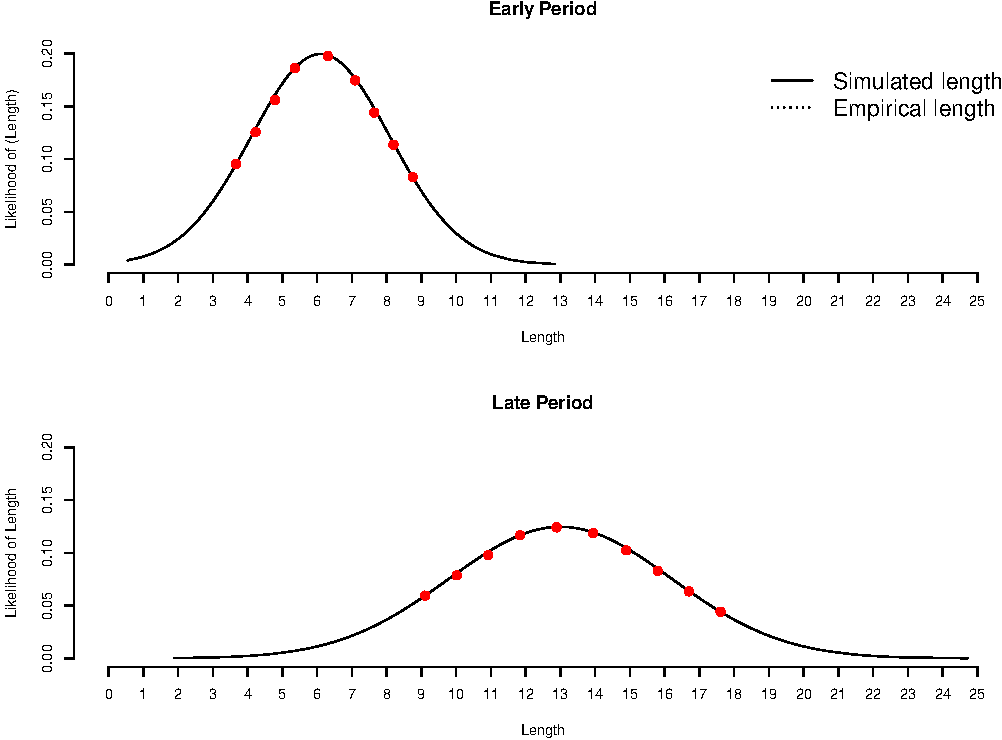
\includegraphics{The-Bayesian-Inferential-Paradigm-in-Archaeology-rmarkdown_files/figure-latex/Fig1-1.pdf}
\caption{Figure 1 Likelihoods of the maximum length data. The red dashed
lines illustrate the ``Normal'' likelihood of the maximum lengths data
measurements obtained empirically from the archaeological Early (top)
and Late (bottom) periods. The likelihood values were obtained after
estimating the parameters of the Normal probability distribution that
maximized the likelihood of the measurement values (i.e., Maximum
Likelihood Estimation, MLE). Following this procedure, we used the MLE
parameter estimates to simulate the likelihood of hypothetical maximum
length values greater than the range observed archaeologically. The
black solid line depicts these values. In both panels, we overlaid the
empirical (gray dotted) over the hypothetical (black solid) likelihood
estimates for comparison}
\end{figure}

Following this exact procedure for the Late Period, the archaeologist
obtained a p-value less than 0.001 for the arrow hypothesis. However,
the \textbf{p}-values for the speartip and dart tip hypotheses are both
greater than 0.05. Therefore, although the archaeologist may reject the
arrow hypothesis, the inference cannot be distinguished between
\emph{``the sample does not have a low probability of resulting from a
population of dart tips''} and \emph{``the sample does not have a low
probability of resulting from a population of spear tips''}.

\hypertarget{bayesian-analysis}{%
\subsubsection{Bayesian analysis}\label{bayesian-analysis}}

\protect\hyperlink{ref-otarola-castillo_bayesian_2018}{Otárola-Castillo
and Torquato}
(\protect\hyperlink{ref-otarola-castillo_bayesian_2018}{2018})'s
archaeologist then compared the NHST analysis to one using a Bayesian
framework. The authors did this to show how archaeologists might apply
Bayesian statistics to assign probabilities to the hypotheses that the
archaeological projectile points were arrows, dart tips, or spear tips -
given the data in hand.

This approach is advantageous when a scientist uses multiple working
hypotheses and is interested in deciding which is most probably
supported by the data. The Bayesian framework can achieve this goal by
using the same assumptions about the underlying probability
distributions as those in the NHST approach. Using Bayes' theorem, one
may then represent prior knowledge as a corresponding prior probability
distribution and calculate each hypothesis's posterior probability.

To conduct this analysis, Otárola-Castillo and Torquato followed the
procedures on likelihoods, prior and posterior probabilities, and MCMC
sampling we outlined in our Bayesian Statistics section above. For
additional technical detail, we refer the reader to the What is Bayes'
Theorem section below. The authors modelled the likelihood of the
maximum projectile length using the ``Normal'' probability model (Figure
1). They also modelled prior knowledge using a uniform probability
distribution to reflect no previous information and demonstrate the
probabilistic approach to hypothesis selection. Under the uniform
distribution, the prior probabilities of all maximum projectile lengths
were identical. Together, the likelihood and prior probability models
are foundational components of Bayesian Inference.

The archaeologist in
\protect\hyperlink{ref-otarola-castillo_bayesian_2018}{Otárola-Castillo
and Torquato}
(\protect\hyperlink{ref-otarola-castillo_bayesian_2018}{2018}) then used
an MCMC procedure to calculate the probability of each hypothesis: that
the archaeological samples were either arrow, dart, or spear, applying a
two-step process. First, they generated samples from the posterior
distribution via MCMC. Second, they compared the sampled values to
intervals defined by one standard deviation around the mean of the
ethnographically observed values for each of the point types (Table 4,
Figure 2). In this way, sampled posterior point lengths that lay between
4.9 cm and 8.9 cm were defined (a posteriori) as Arrows; those in the
range 9 to 13 cm Darts; those in 12 to 16 cm Spears. Point lengths
outside the range of 4.6 to 16 cm were outside of the evaluated
hypotheses. Therefore, they were declared to belong to a group labelled
``Other.'' There is some overlap between the summary probability
distributions implied by the ethnographic data. Thus, the hypotheses are
not mutually exclusive. In other words, due to overlapping measurements,
some projectile points may be consistent with more than one hypothesis.
We discuss the implications of this overlap below.

Next, the archaeologist calculated the posterior probabilities by
dividing the number of projectile points consistent with each hypothesis
by the total number of projectile points for each period. The posterior
probability of point lengths for each hypothesis is reported in Table 4
and illustrated in Figure 2. Since the hypotheses are non-mutually
exclusive, the posterior probabilities corresponding to each hypothesis
within a period are not expected to sum to 1. Depending on one's
hypotheses, the interpretation of probabilities relating to non-mutually
exclusive outcomes may be problematic. For example, one might ask, what
is the probability that the projectile points are Arrows or Darts? In
this case, because some Arrows may be similar in length to Darts, these
are not mutually exclusive outcomes, and one may not simply add their
respective probabilities together. The solution is to use the General
Addition Rule of probability (see
\protect\hyperlink{ref-diez_open_2019}{Diez, Barr, and Cetinkaya-Rundel}
(\protect\hyperlink{ref-diez_open_2019}{2019}): 83-88). We do not
evaluate such an hypothesis in this example but note this rule so that
readers may adopt it if needed for their own work.

Using the resulting Bayesian posterior probability distribution to
conduct inference lets scientists make fully probabilistic statements
about their hypotheses and thus make more explicit comparisons than
those provided by the NHST framework. The results highlighted by Figure
2 seem clear regarding the probability of each hypothesis. We will
discuss these further. After examining the resulting posterior
probabilities, the archaeologist determined that the Early period sample
points were most probably used as arrows (with probability 0.97) and
likely propelled by a bow-like mechanism. This mode of stone point
propelling changed during the Late Period when the people living on this
site began to use mainly hand-thrown spears (with probability 0.89).

In this way, the Bayesian approach to testing hypotheses leads to
results that are more readily interpreted than those via the p-value
based NHST. In particular, we are provided with measures of probability
that the data support the hypotheses, which have considerably more
intuitive interpretation than those provided by p-values.

\newpage

\begin{quote}
\textbf{Table 4} \emph{Posterior probabilities that the Early and Late
Period maximum projectile point lengths were associated with arrow,
dart, and spear propelling technologies.}
\end{quote}

\begin{longtable}[]{@{}llll@{}}
\toprule
Function & Mean±SD of max. point length & Early Period & Late Period \\
\midrule
\endhead
Arrow & 6.9 ± 2 & 0.97 & 0.0009 \\
Dart Tips & 11 ± 2 & 0.004 & 0.17 \\
Spear Tips & 14 ± 2 & 0.00002 & 0.89 \\
\bottomrule
\end{longtable}

\begin{figure}
\centering
\includegraphics{The-Bayesian-Inferential-Paradigm-in-Archaeology-rmarkdown_files/figure-latex/Fig2-1.pdf}
\caption{Bayesian posterior probability distributions of each of three
propelling technology hypotheses: a) Arrow, b) Dart, c) Spear in the
Early (bottom) and Late (top) periods. The amount of area under the
curve reflects the probability of each hypothesis expressed as
percentages.}
\end{figure}

\newpage

\hypertarget{what-is-bayes-theorem}{%
\subsection{\texorpdfstring{\hfil WHAT IS BAYES'
THEOREM\hfil}{WHAT IS BAYES' THEOREM}}\label{what-is-bayes-theorem}}

Bayes' theorem is an algorithm for obtaining the value of a conditional
probability statement, when one knows its inverse. It is usually
exemplified by considering two related events, A and B. Put simply,
Bayes' theorem states that (equation 1):

\begin{equation}
P(A|B) = \frac{P(B|A)\cdot P(A)}{P(B)}
\label{eg:1}
\end{equation}

In this case, to obtain the conditional probability of A given B,
P(A\textbar B) - here P represents probability and \textbar{} is read as
`given' - one needs to divide the joint probability of A and B, P(A and
B), by the marginal probability of B, P(B). The product of
P(B\textbar A) and P(A) is the joint probability P(A and B). The formula
then generalizes to equation (2):

\begin{equation}
P(A|B) = \frac{P(A \cap B)}{P(B)}
\label{eg:2}
\end{equation}

where the joint probability is divided by the marginal P(B).
Statisticians call P(A\textbar B) the posterior probability of A given
B, P(B\textbar A) the inverse conditional (or likelihood) of B given A,
and P(A) the prior probability of A.

\hypertarget{the-link-between-bayes-theorem-inference-data-and-hypotheses}{%
\subsubsection{The link between Bayes' theorem, inference, data and
hypotheses}\label{the-link-between-bayes-theorem-inference-data-and-hypotheses}}

The simulated archaeological scenario above provided a tangible example
of the different components of a Bayesian analysis, including an event's
probability, the probability of one event given another, prior and
posterior probabilities. Although the procedure here is specific to
archaeological data, Bayes' theorem is a very general algorithm that is
useful for a wide variety of data and data-generating processes. This
section generalizes Bayes' theorem to a variety of other scenarios.

We stated earlier that Bayesian statistics uses the data in hand, (D),
to assign probabilities to hypotheses about a population (H). The
statement P(H\textbar D), i.e., the probability of the hypothesis given
the data, formalizes this relationship. To operationalize this statement
in the context of data and hypotheses, Bayes' theorem functions as

\begin{equation}
P(H|D) = \frac{P(D|H)\cdot P(H)}{P(D)}
\label{eg:3}
\end{equation}

where: P(H\textbar D) is the posterior probability --- the probability
of the hypothesis given the data in hand; P(D\textbar H) is the
probability of the data given the hypothesis, or the ``likelihood'' of
the observed data; P(H) is the prior probability of the hypothesis
(before the data were observed), and P(D) is the probability of the data
in hand (out of all possible values of the data). Alternatively, using
modern statistical vernacular this operation can then be expressed in a
slightly different form as:

\begin{equation}
Posterior  = \frac{Likelihood \cdot Prior}{P(Data)}
\label{eg:4}
\end{equation}

In Otárola-Castillo and Torquato's artificial example, the hypotheses
represented the belief that the observed Early and Late period
projectile point data represented samples from populations derived from
particular propelling technologies. The data were modelled by the Normal
probability distribution, and the hypotheses were characterized by the
values of the model's parameters.

We use the symbol x to represent the observed data and the symbol
\(\theta\) to represent the parameter(s) of our model of the population
that we are trying to learn about. Given x and a model with parameter(s)
\(\theta\), we can more formally describe Bayes' theorem and its three
components: the \emph{likelihood}, the \emph{prior}, and the
\emph{posterior}.

\begin{enumerate}
\def\labelenumi{\roman{enumi}.}
\item
  The \emph{likelihood} is a statistical function. Its form is
  determined by the specific probability model we are using but, in
  general terms it is represented by P(x\textbar{}\(\theta\)).
  Consequently, the likelihood is the probability of observing
  particular data values given some specific values of the unknown
  parameters. Thus, this is a formal statement of the relationship
  between what we want to learn and the data we collect.
\item
  The \emph{prior} is also a function and can be represented by
  P(\(\theta\)). In simple terms, we can think of this as the
  probability we attach to observing specified values of the unknown
  parameters before (\emph{a priori}) we observe the data. In other
  words, this is a formal statement of what we knew before the latest
  data were collected.
\item
  The posterior is the probability distribution that we want to obtain
  (a combination of the information contained in the data, the
  likelihood and the prior) and can be represented by
  P(\(\theta\)\textbar x). Put plainly, this is the probability we
  attach to specified values of the unknown parameters after observing
  the data. In this more technical context, we can express Bayes'
  theorem as:
\end{enumerate}

\begin{equation}
P(\theta|x) = \frac{P(x|\theta)\cdot P(\theta)}{P(x)}
\label{eg:5}
\end{equation}

In addition, the numerator, the product of the likelihood and the prior
probability without the normalizing denominator P(\emph{x})is
proportional to (\(\propto\)) the posterior and is often computed and
expressed by

\begin{equation}     
P(\theta|x) \propto P(x| \theta) \cdot P(\theta)
\label{eg:6}
\end{equation}

or,

\begin{equation}
Posterior \propto Likelihood \cdot Prior
\label{eg:7}
\end{equation}

In this manner, Bayesian statistics offers an alternative statistical
framework for evaluating hypotheses through a mechanism for obtaining
\emph{a posteriori} information about the parameter values of interest,
based upon the data, a model, and appropriately formulated prior
information. In other words, given an explicit statement of our \emph{a
priori} information, a clearly defined statistical model and a desire to
obtain \emph{a posteriori} understanding, Bayes' theorem provides us
with a probabilistic framework within which to make interpretations.

In addition to the coherent and explicit nature of the framework, there
is another attractive feature of adopting the Bayesian paradigm in that
it allows us to learn from experience. Priors enable the explicit
contextualization of previous knowledge or beliefs about the topic under
investigation (\protect\hyperlink{ref-cowgill_distinguished_1993}{George
L. Cowgill 1993}; \protect\hyperlink{ref-buck_bayesian_1996}{Caitlin E.
Buck, Cavanagh, and Litton 1996}). This should be a natural feature to
archaeologists for whom context is quite meaningful, or as
\protect\hyperlink{ref-buck_bayesian_1996}{Caitlin E. Buck, Cavanagh,
and Litton} (\protect\hyperlink{ref-buck_bayesian_1996}{1996}) discuss,
archaeologists interpret the discovery of new artifacts in conjunction
with artifacts that have already been discovered.

Moreover, today's posterior information (based on current data and prior
information) is in a suitable form to become the prior for further work
if and when more data become available. Few other interpretative
frameworks offer a clear structure for updating one's beliefs in the
light of new information and yet it is such an important part of most
intuitive approaches to learning about the world in which we live.
\newpage

\hypertarget{other-archaeological-applications}{%
\subsection{\texorpdfstring{\hfil OTHER ARCHAEOLOGICAL
APPLICATIONS\hfil}{OTHER ARCHAEOLOGICAL APPLICATIONS}}\label{other-archaeological-applications}}

\hypertarget{chronological-modelling}{%
\subsubsection{Chronological modelling}\label{chronological-modelling}}

The reliable construction of chronologies is an integral part of all
archaeological research. Consequently, an abundance of research has been
conducted to create robust chronologies and thus, assist archaeologists
in interpreting past events. Early work laid the foundation for the use
of Bayesian methods in chronological modelling to improve precision
(\protect\hyperlink{ref-naylor_archaeological_1988}{Naylor and Smith
1988}; \protect\hyperlink{ref-buck_combining_1991}{Caitlin E. Buck et
al. 1991}; \protect\hyperlink{ref-buck_calibration_1992}{Caitlin E.
Buck, Litton, and Smith 1992}). The advent and continued improvement of
user-friendly modelling software, including BCal
(\protect\hyperlink{ref-buck_bcal_1999}{Caitlin E. Buck, Christen, and
James 1999}) and OxCal
(\protect\hyperlink{ref-bronk_ramsey_analysis_1994}{Bronk Ramsey 1994},
\protect\hyperlink{ref-bronk_ramsey_methods_2017}{2017}), has enabled
many archaeologists to employ Bayesian chronological modelling in their
research. In fact, the construction of chronologies has been described
as the one archaeological application of Bayesian methods that is now
routine (\protect\hyperlink{ref-buck_being_2015}{Caitlin E. Buck and
Meson 2015}).

There has been a documented increase in the use of Bayesian
chronological modelling over the last decade
(\protect\hyperlink{ref-bayliss_quality_2015}{Bayliss 2015};
\protect\hyperlink{ref-hamilton_myths_2018}{Hamilton and Krus 2018}), as
numerous studies have re-examined radiocarbon dates to refine regional
chronologies. Although these methods were initially used by
archaeologists in the United Kingdom
(\protect\hyperlink{ref-hamilton_myths_2018}{Hamilton and Krus 2018}),
Bayesian chronological studies have now been conducted in nearly every
region of archaeological interest, including:

\begin{enumerate}
\def\labelenumi{\roman{enumi}.}
\tightlist
\item
  Central America
  (\protect\hyperlink{ref-inomata_high-precision_2017}{Inomata et al.
  2017}; \protect\hyperlink{ref-mendelsohn_chronology_2018}{Mendelsohn
  2018}; \protect\hyperlink{ref-tsukamoto_building_2020}{Tsukamoto et
  al. 2020});
\item
  South America (\protect\hyperlink{ref-marsh_dating_2017}{Erik J. Marsh
  et al. 2017}; \protect\hyperlink{ref-wynveldt_late_2017}{Wynveldt et
  al. 2017}),
\item
  Europe (\protect\hyperlink{ref-arvaniti_tracing_2018}{Arvaniti and
  Maniatis 2018}; \protect\hyperlink{ref-jimenez_cultural_2018}{Jiménez
  et al. 2018}; \protect\hyperlink{ref-krajcarz_towards_2018}{Krajcarz
  et al. 2018}; \protect\hyperlink{ref-manning_new_2018}{Manning et al.
  2018}; \protect\hyperlink{ref-ricci_chronological_2018}{Ricci et al.
  2018}; \protect\hyperlink{ref-paulsson_radiocarbon_2019}{Paulsson
  2019}),
\item
  Asia (\protect\hyperlink{ref-long_bayesian_2017}{Long, Wagner, and
  Tarasov 2017}; \protect\hyperlink{ref-ricci_chronological_2018}{Ricci
  et al. 2018};
  \protect\hyperlink{ref-birch-chapman_bayesian_2019}{Birch-Chapman and
  Jenkins 2019}; \protect\hyperlink{ref-yang_refined_2019}{Yang et al.
  2019}),
\item
  Africa (\protect\hyperlink{ref-kramer_sibling_2016}{Kramer, Veile, and
  Otárola-Castillo 2016}; \protect\hyperlink{ref-brandt_new_2017}{Brandt
  et al. 2017}; \protect\hyperlink{ref-sadr_new_2017}{Sadr et al. 2017};
  \protect\hyperlink{ref-loftus_archaeological_2019}{Loftus, Mitchell,
  and Bronk Ramsey 2019}), and
\item
  Oceania (\protect\hyperlink{ref-brockwell_new_2017}{Brockwell et al.
  2017}; \protect\hyperlink{ref-kirch_new_2017}{Kirch and Swift 2017};
  \protect\hyperlink{ref-urwin_chronology_2018}{Urwin and Arifeae 2018};
  \protect\hyperlink{ref-david_dating_2019}{David et al. 2019}).
\end{enumerate}

Indeed, even those archaeologists who simply report individual,
calibrated radiocarbon dates are now reliant on Bayesian methods since
the most recent estimates of the radiocarbon calibration curves
(IntCal20, SHCal20, and Marine20) are grounded in Bayesian inference.
They were constructed using a Bayesian spline approach to combine data
from tree rings, floating tree-ring chronologies, lacustrine and marine
sediments, speleothems, and corals
(\protect\hyperlink{ref-reimer_intcal20_2020}{Reimer et al. 2020}).

Archaeologists have applied Bayesian methods to other methods of
absolute dating. For example, recent studies have constructed
chronological models using optically-stimulated luminescence (OSL) dates
(\protect\hyperlink{ref-clarkson_human_2017}{Clarkson et al. 2017};
\protect\hyperlink{ref-combes_bayesian_2017}{Combès and Philippe 2017};
\protect\hyperlink{ref-veth_early_2017}{Veth 2017};
\protect\hyperlink{ref-jimenez_cultural_2018}{Jiménez et al. 2018};
\protect\hyperlink{ref-demuro_corrigendum_2019}{Demuro et al. 2019};
\protect\hyperlink{ref-heydari_bayesian_2020}{Heydari et al. 2020}), and
dendrochronology (\protect\hyperlink{ref-millard_bayesian_2002}{Millard
2002}; \protect\hyperlink{ref-hassan_simple_2019}{Hassan, Jones, and
Buck 2019};
\protect\hyperlink{ref-lorentzen_shipbuilding_2020}{Lorentzen, Manning,
and Cvikel 2020}).

Perhaps most significantly, Bayesian chronological modelling enables
archaeologists to include numerous sources of archaeological dates in a
single interpretive framework, including those drawn from relative
dating and absolute dating, to create chronologies of hard-to-date
contexts. By combining relative dating and absolute dating methods with
Bayesian modelling, archaeologists can produce more precise and accurate
dates (\protect\hyperlink{ref-cowgill_we_2015}{George L. Cowgill 2015}).
For example, \protect\hyperlink{ref-croix_dating_2019}{Croix et al.}
(\protect\hyperlink{ref-croix_dating_2019}{2019}) combined artifact
chronologies, coin dates, and radiocarbon dating in a Bayesian model to
date earthworks in Denmark. Prior to this research, dating these
structures was difficult due to the limited survival of dateable
artifacts and the reuse of building materials in antiquity. By
constructing a Bayesian chronological model using coin age and
radiocarbon dates, researchers improved the dating precision of the
earthworks. Furthermore,
\protect\hyperlink{ref-dinapoli_model-based_2020}{DiNapoli et al.}
(\protect\hyperlink{ref-dinapoli_model-based_2020}{2020}) used a
Bayesian modelling approach to combine radiocarbon dates, stratigraphy,
and ethnohistoric accounts to examine the collapse and resilience of
populations on Rapa Nui. Other examples of studies include those
combining absolute dating methods (e.g.,
\protect\hyperlink{ref-anyon_re-evaluating_2017}{Anyon et al. 2017};
\protect\hyperlink{ref-fitzsimmons_chronological_2017}{Fitzsimmons et
al. 2017}; \protect\hyperlink{ref-smith_puntutjarpa_2017}{Smith,
Williams, and Ross 2017}) and those drawing on relative and absolute
dating methods (e.g.,
\protect\hyperlink{ref-guerin_chronology_2017}{Guérin et al. 2017};
\protect\hyperlink{ref-douka_age_2019}{Douka et al. 2019}).

Other studies have used Bayesian modelling to clarify the complex
relationship between humans and the environment. For example, Banks and
colleagues (2019) utilized Bayesian hierarchical modelling to determine
the date for cultures from Upper Palaeolithic France. These dates were
then compared to palaeoecological records to determine the
palaeoclimatic variability during each period. Similarly,
\protect\hyperlink{ref-kearney_vegetation_2019}{Kearney}
(\protect\hyperlink{ref-kearney_vegetation_2019}{2019}) used Bayesian
methods to combine archaeological and palaeoecological chronologies in a
study examining the connection between vegetation changes and human
activity near a megalithic tomb dating to the Neolithic in Ireland.
Using this method, he was able to determine if significant palynological
events occurred before, after or during the construction and use of the
tomb. Ultimately, he determined that the clearing of the woodland
occurred prior to the construction of the megalith.

\hypertarget{artifact-analysis}{%
\subsubsection{Artifact analysis}\label{artifact-analysis}}

Bayesian inference has been applied in numerous ways to study a broad
array of artifacts, including ceramics, bone and stone tools. Early
applications examined the provenance of artifacts and ceramic seriation
(e.g., \protect\hyperlink{ref-buck_computational_1990}{Caitlin E. Buck
and Litton 1990}; \protect\hyperlink{ref-buck_bayesian_1996}{Caitlin E.
Buck, Cavanagh, and Litton 1996};
\protect\hyperlink{ref-halekoh_bayesian_1999}{Halekoh and Vach 1999};
\protect\hyperlink{ref-robertson_spatial_1999}{Robertson 1999}).
Continued research examining ceramics has utilized Bayesian modelling of
radiocarbon dates to determine the chronologies of ceramic artifacts by
combining absolute dating and studies of ceramic typologies (e.g.,
\protect\hyperlink{ref-naylor_archaeological_1988}{Naylor and Smith
1988}). Similar methods have been used to examine ceramic traditions in
Europe (\protect\hyperlink{ref-krol_chronology_2020}{Krol, Dee, and
Nieuwhof 2020}), Bolivia
(\protect\hyperlink{ref-marsh_temporal_2019}{Erik J. Marsh et al.
2019}), Guatemala (\protect\hyperlink{ref-arroyo_refining_2020}{Arroyo
et al. 2020}), and Papua New Guinea
(\protect\hyperlink{ref-skelly_changing_2018}{Skelly et al. 2018}). The
combination of chronological modelling and ceramic data has been used to
examine the dispersal and spread of ceramic cultures (e.g.,
\protect\hyperlink{ref-mehault_applying_2017}{Méhault 2017};
\protect\hyperlink{ref-binder_modelling_2018}{Binder et al. 2018}).

Recently, the application of Bayesian modelling to ceramic analysis has
extended beyond seriation. For example,
\protect\hyperlink{ref-fernandes_reconstruction_2018}{Fernandes et al.}
(\protect\hyperlink{ref-fernandes_reconstruction_2018}{2018}) used a
Bayesian approach to identify the types of food that created residues in
prehistoric European pottery. By analysing carbon isotope measurements
and comparing them with measurements from known sources, the authors
determined which foods had contributed to the residues and thus how the
pots had been used. Since pots are reused to prepare multiple types of
foods, results can be ambiguous when identifying the foods contributing
to residues. The use of Bayesian methods addressed this ambiguity by
estimating the contribution of various food types to the residues.

Furthermore, Bayesian methods are becoming integral in the study of
stone and bone tools. Researchers have used Bayesian methods to test
hypotheses about stone tool assemblages (e.g.,
\protect\hyperlink{ref-marwick_early_2016}{Marwick et al. 2016}) and
develop techniques for studying stone tools. These techniques allow
researchers to assign probabilities to the phenomenon being studied. For
example, \protect\hyperlink{ref-murray_new_2020}{Murray et al.}
(\protect\hyperlink{ref-murray_new_2020}{2020}) developed a novel method
combining 3D microscopic analyses of surface roughness and a Bayesian
probability model to evaluate if Middle Stone Age silcrete tools from
Pinnacle Point 13B (South Africa) had been heat treated. The model
measured the probability that a tool has been heat treated,allowed for
the continued updating from future heat treatment experiments, and
performed with high accuracy. Similarly, other researchers combined a
taphonomic analysis of the surface of unworked bone and bone tools with
multivariate Bayesian modelling to quantify the taphonomic changes on
the surfaces of the unworked and worked bones to accurately predict the
original surface of the bone tools
(\protect\hyperlink{ref-martisius_time_2018}{Martisius et al. 2018},
\protect\hyperlink{ref-martisius_method_2020}{2020}).

\hypertarget{zooarchaeology}{%
\subsubsection{Zooarchaeology}\label{zooarchaeology}}

Researchers have used Bayesian statistics to study zooarchaeological
trends. Pioneering work by
\protect\hyperlink{ref-fisher_mastodont_1987}{D. C. Fisher}
(\protect\hyperlink{ref-fisher_mastodont_1987}{1987}) used Bayesian
inference to determine whether scavenging or hunting led to the creation
of butchery marks on proboscidean assemblages. Recent work has focused
on studying seasonality and domestication. For example,
\protect\hyperlink{ref-parkington_contemporaneity_2020}{Parkington et
al.} (\protect\hyperlink{ref-parkington_contemporaneity_2020}{2020})
used a Bayesian approach to study the seasonal use of Later Stone Age
archaeological sites in South Africa. By reanalysing their previous
studies on the timing of death using a Bayesian framework, they were
able to determine, with greater accuracy, when hunter-gatherers would
have used the sites where seal remains were found. Additionally,
scholars have used Bayesian methods to construct phylogenies examining
the domestication of animals, including swamp buffalo
(\protect\hyperlink{ref-wang_whole_2017}{Wang et al. 2017}) and pigs
(\protect\hyperlink{ref-xiang_origin_2017}{Xiang et al. 2017}). Other
research has examined the foods consumed by domesticated animals.
\protect\hyperlink{ref-blanz_identifying_2020}{Blanz et al.}
(\protect\hyperlink{ref-blanz_identifying_2020}{2020}) used Bayesian
modelling to examine the diets of modern sheep, specifically the amount
of seaweed consumed, which can be used as a reference sample for
identifying similar consumption patterns in archaeological contexts.

Additionally, archaeologists have used Bayesian methods to study faunal
assemblages and make inferences about their use. For example,
\protect\hyperlink{ref-osborn_bayesian_2019}{Osborn}
(\protect\hyperlink{ref-osborn_bayesian_2019}{2019}) constructed a
Bayesian network model using ethnographic, ethnohistoric, and
archaeological data to determine whether Andean faunal assemblages
indicated feasting, sacrifice, or daily refuse. The primary benefit of
using a Bayesian approach in the study was the resulting replicable
analysis that eliminates the subjectivity present in interpreting faunal
assemblages. Rather, this method reports the probabilities of the faunal
assemblage representing each type of behaviour. Furthermore,
\protect\hyperlink{ref-baumann_role_2020}{Baumann et al.}
(\protect\hyperlink{ref-baumann_role_2020}{2020}) used Bayesian methods
to estimate the abundance of foxes and hares in Palaeolithic Europe to
determine how their abundance changed over time as they were hunted by
humans for their meat, fur, and teeth. The use of Bayesian methods in
this study allowed the researchers to overcome a small sample size while
modelling animal abundance.

Bayesian techniques have been used to develop and re-examine the methods
used in zooarchaeological research. Researchers have used Bayesian
inference to develop a reliable and replicable probabilistic method to
distinguish between sheep and goat bones in archaeological contexts
(\protect\hyperlink{ref-wolfhagen_probabilistic_2017}{Wolfhagen and
Price 2017}). Since goats and sheep are very similar species that share
many traits, it can be difficult to distinguish between them. This
method provides the probability that a specimen is a goat given the
identified traits. Furthermore,
\protect\hyperlink{ref-wolfhagen_re-examining_2020}{Wolfhagen}
(\protect\hyperlink{ref-wolfhagen_re-examining_2020}{2020}) has
re-examined the ``logarithm size index'' (LSI), a method for comparing
the body sizes of animals between assemblages that is typically used in
studies of animal domestication. He suggests adopting Bayesian
multilevel LSI models to examine hypotheses about faunal assemblages.

\hypertarget{bioarchaeology}{%
\subsubsection{Bioarchaeology}\label{bioarchaeology}}

The use of Bayesian methods in bioarchaeological analyses was pioneered
by Konigsberg and colleagues for studying age-at-death and stature
estimation (e.g.,
\protect\hyperlink{ref-konigsberg_estimation_1992}{Lyle W. Konigsberg
and Frankenberg 1992};
\protect\hyperlink{ref-konigsberg_paleodemography_1994}{Lyle W.
Konigsberg and Frankenberg 1994};
\protect\hyperlink{ref-lucy_bayesian_1996}{Lucy et al. 1996};
\protect\hyperlink{ref-konigsberg_stature_1998}{Lyle W. Konigsberg et
al. 1998}). Recent research has continued to apply Bayesian statistics
to the construction of biological profiles. For example,
\protect\hyperlink{ref-anzellini_estimating_2019}{Anzellini and Toyne}
(\protect\hyperlink{ref-anzellini_estimating_2019}{2019}) proposed the
use of Bayesian logistic regression to account for uncertainty in the
sample when estimating the sex of individuals found in commingled
contexts in the Andes. Although the frequentist and Bayesian approaches
produced similar results, the authors demonstrated the validity of using
Bayesian methods to account for uncertainty and to produce usable
demographic profiles in bioarchaeological studies. Furthermore,
\protect\hyperlink{ref-rosenstock_human_2019}{Rosenstock et al.}
(\protect\hyperlink{ref-rosenstock_human_2019}{2019}) used Bayesian
additive mixed modelling to examine the global spatiotemporal trend in
stature. This method enabled the researchers to account for
spatiotemporally patchy data as well as fragmentary skeletal samples.

Further studies have utilized Bayesian mixing models to reconstruct
prehistoric diets. Typically, these methods have used carbon and
nitrogen stable isotope data to determine the types of foods people were
eating. One popular method is called the Food Reconstruction Using
Isotopic Transferred Signals (FRUITS) approach, which can account for
multiple dietary sources and the uncertainty inherent in dietary
inference. For example,
\protect\hyperlink{ref-pezo-lanfranco_middle_2018}{Pezo-Lanfranco et
al.} (\protect\hyperlink{ref-pezo-lanfranco_middle_2018}{2018}) used
Bayesian mixing models to quantify the proportion of three sources of
food: plants, marine mammals, and terrestrial mammals. They determined
that the people of the Atlantic Forest of South America consumed a large
amount of carbohydrates, suggesting a unique diet compared to other
populations in the area during the Middle Holocene. Using various
Bayesian mixing models, other studies have examined prehistoric dietary
trends in Europe (\protect\hyperlink{ref-bownes_using_2017}{Bownes et
al. 2017};
\protect\hyperlink{ref-sjogren_modelling_2017}{\textbf{sjogren\_modelling\_2017?}};
\protect\hyperlink{ref-boethius_fish_2018}{Boethius and Ahlström 2018};
\protect\hyperlink{ref-cubas_long-term_2019}{Cubas et al. 2019}), South
America (\protect\hyperlink{ref-gordon_dietary_2018}{Gordón et al.
2018}), and Africa
(\protect\hyperlink{ref-maurer_geochemical_2017}{Maurer et al. 2017}).
Recent studies have used similar Bayesian modelling to study prehistoric
weaning trends (\protect\hyperlink{ref-king_comparison_2017}{King et al.
2017}). Specifically, using the FRUITS method,
\protect\hyperlink{ref-de_angelis_dietary_2020}{De Angelis et al.}
(\protect\hyperlink{ref-de_angelis_dietary_2020}{2020}) reconstructed
the diet of those buried at the Quarto Cappello del Prete. From this
reconstruction, they determined that Roman children were weaned around
three years of age.

Other researchers have used mixed/multilevel/hierarchical modelling
approaches. For example,
\protect\hyperlink{ref-perri_dietary_2019}{Perri et al.}
(\protect\hyperlink{ref-perri_dietary_2019}{2019}) examined the canine
diet as a proxy for human diets in archaeological contexts in Nicaragua.
To infer the probability of the model's parameters the authors used a
Bayesian approach including MCMC to estimate the denominator of Bayes
theorem. Hierarchical models in this context are flexible and scalable
(\protect\hyperlink{ref-gelman_data_2006}{Gelman and Hill 2006}). They
can include individual and group level data in a model. This flexibility
provides improved inference on the parameters in question, resulting in
more accurate estimates of the model's parameters
(\protect\hyperlink{ref-katahira_how_2016}{Katahira 2016}).

\hypertarget{spatial-archaeology}{%
\subsubsection{Spatial archaeology}\label{spatial-archaeology}}

By combining prior knowledge regarding geographical data, archaeologists
have been able to study spatial trends (see Chapter xx). For example,
researchers have used Bayesian methods to examine the placement of
archaeological sites on the landscape
(\protect\hyperlink{ref-wright_analysis_2014}{Wright, MacEachern, and
Lee 2014}) and predict the locations and settlement patterns of
archaeological sites
(\protect\hyperlink{ref-ortman_empirical_2007}{Ortman, Varien, and Gripp
2007}; \protect\hyperlink{ref-stewart_novel_2017}{Stewart et al. 2017}).
Other research has incorporated Bayesian chronological modelling into
spatial archaeological analyses. For example,
\protect\hyperlink{ref-snitker_patch-based_2018}{Snitker et al.}
(\protect\hyperlink{ref-snitker_patch-based_2018}{2018}) combined
prehistoric land use maps generated by surveys, chronological data, and
Bayesian methods to examine shifting occupation and land use patterns in
Spain. The use of Bayesian methods in this study was critical as it
allowed the researchers to make probabilistic inferences regarding the
most likely occupation period at archaeological sites that may have been
reused throughout history. Similarly,
\protect\hyperlink{ref-wright_spatial_2020}{Wright et al.}
(\protect\hyperlink{ref-wright_spatial_2020}{2020}) used Bayesian
chronological modelling of radiocarbon dates to construct a summed
probability distribution estimating occupation events in the Baekje
Kingdom of Korea during the Three Kingdoms Period (57 BCE to 688 CE).
The researchers proceeded to use these data as part of a larger model
examining the spatial distribution and dynamics of human activity areas
over time. These methods allowed the researchers to make probabilistic
statements about settlement patterns' hypotheses at a time when
occupation patterns were thought to be changing. \newpage

\hypertarget{some-practicalities}{%
\subsection{\texorpdfstring{\hfil SOME
PRACTICALITIES\hfil}{SOME PRACTICALITIES}}\label{some-practicalities}}

\hypertarget{modelling}{%
\subsubsection{Modelling}\label{modelling}}

Although numerous probability models exist, many archaeological problems
are statistically non-standard. This has often meant that the close
collaboration of a number of specialists, including statisticians, is
required to build useful models. Fortunately, statisticians have often
found archaeological problems to be interesting and challenging and so
this kind of collaboration is not too unusual. Nonetheless, although
applications of Bayesian analysis to archaeology have been around for
more than 30 years, they are by no means ubiquitous and further
collaboration is certainly needed.

\hypertarget{specifying-the-prior}{%
\subsubsection{Specifying the prior}\label{specifying-the-prior}}

One of the major stumbling blocks to the more widespread use of Bayesian
techniques in archaeology is the perceived difficulty of specifying
prior information. Some archaeologists do not acknowledge that reliable
prior information exists and others have philosophical objections to the
use of subjective opinions in formal inference. Both such groups
typically prefer to continue using exploratory methods or traditional
NHST-based ones. Others have expert knowledge and would like to use it,
but have difficulty expressing their ideas in a suitable form because of
their lack of knowledge about the mathematics that underlie the models
they wish to use. Tackling this problem requires further collaboration,
clear communication, and an acceptance that different researchers will
have varying views on which interpretive framework to use or which
specific model to adopt. Most importantly, there is no need for everyone
to agree. Researchers who adopt the Bayesian framework are forced to be
explicit about what they believe. As a result, different workers can
compute posteriors based on their own prior information and compare them
formally with the inferences of others.

\hypertarget{evaluating-the-posteriors}{%
\subsubsection{Evaluating the
posteriors}\label{evaluating-the-posteriors}}

Early applications of the Bayesian framework to archaeology (as with
other disciplines) were restricted to likelihoods and priors for which
the necessary calculations could easily be undertaken. However, since
the mathematical integrations required for some models are not
analytically soluble, a fair number of real questions simply could not
be tackled. These problems have now largely been overcome by the
widespread adoption of numerical techniques that allow the posterior
information to be sampled rather than obtained exactly. Some of the
earliest illustrations of the use of these techniques for evaluating
Bayesian posteriors were in Bayesian radiocarbon calibration
(\protect\hyperlink{ref-buck_calibration_1992}{Caitlin E. Buck, Litton,
and Smith 1992}; \protect\hyperlink{ref-buck_bcal_1999}{Caitlin E. Buck,
Christen, and James 1999};
\protect\hyperlink{ref-litton_archaeological_1996}{Litton and Buck
1996}). Advances in algorithms to create and sample from Markov chain
Monte Carlo simulations (MCMC) such as Metropolis-Hastings, Gibbs
sampling, and the Hamiltonian procedures such as No U-Turn Sampling
(NUTS) (e.g., \protect\hyperlink{ref-dunson_hastings_2020}{Dunson and
Johndrow 2020}; \protect\hyperlink{ref-hoffman_no-u-turn_2014}{Hoffman
and Gelman 2014}) implemented by popular software like BUGS, JAGS, and
STAN (\protect\hyperlink{ref-gilks_language_1994}{Gilks, Thomas, and
Spiegelhalter 1994}; \protect\hyperlink{ref-plummer_jags_2003}{Plummer
2003}; \protect\hyperlink{ref-sturtz_r2winbugs_2005}{Sturtz, Ligges, and
Gelman 2005}; \protect\hyperlink{ref-team_rstan_2019}{Team 2019}) have
helped to alleviate this problem.

\hypertarget{interpretation}{%
\subsubsection{Interpretation}\label{interpretation}}

Ultimately, the most important part of any statistical investigation is
the interpretation of the results obtained. The posterior distributions
that arise from Bayesian analyses can be very complex and are sometimes
not directly interpretable in terms of the original problem. This means
that exploratory methods of data analysis may be needed to help
investigate, interpret, and report upon the posterior distributions
obtained. When making such interpretations, the level of confidence in
the posteriors is affected by their sensitivity to changes in the data,
priors, or model. Such sensitivity should be investigated as part of the
interpretation of all posterior information. It is always useful to
relax some of the prior assumptions and re-compute the posteriors to see
what effect this has. All reports of Bayesian analyses should make
reference to sensitivity analyses of this type, since without them we
cannot be sure how robust the results are and thus how reliable they
would be as prior information for future research. \newpage

\hypertarget{hopes-for-the-future}{%
\subsection{\texorpdfstring{\hfil HOPES FOR THE
FUTURE\hfil}{HOPES FOR THE FUTURE}}\label{hopes-for-the-future}}

We have discussed the positive contributions of Bayesian inference to
archaeological thinking. In addition to providing a fully probabilistic
framework, Bayesian statistics requires that one makes existing prior
knowledge explicit to use in statistical analyses. By doing so,
scientists take advantage of a more comprehensive set of information
when evaluating hypotheses. This is a major advantage over NHST and the
related Maximum Likelihood, and Information Theory approaches to
model-selection (\protect\hyperlink{ref-murtaugh_defense_2014}{Murtaugh
2014}). Increases in the popularity of Bayesian applications in
archaeology are likely due to the recognition of these features. To
continue this trend, we outline an ambitious set of initiatives we hope
to see in the future of Bayesian applications in archaeology.

\hypertarget{a-framework-for-archaeological-science}{%
\subsubsection{A framework for archaeological
science}\label{a-framework-for-archaeological-science}}

The Bayesian approach provides a systematic learning procedure, using
evidence to update one's beliefs or hypotheses until reaching a
confident and accurate level of knowledge. This evidence-based learning
approach inherently resembles the scientific process of hypothesis
generation and evaluation. As a science, data-laden inference about the
past is also inherent to archaeology. New knowledge from archaeological
data recovery through excavation, survey, or analytical activities
constantly update archaeologists' state of knowledge and revise the
degree of support for prior hypotheses (e.g., the initial colonization
of the Americas and out of Africa origins of \emph{Homo sapiens}).

\hypertarget{increase-diversity-of-bayesian-applications}{%
\subsubsection{Increase diversity of Bayesian
applications}\label{increase-diversity-of-bayesian-applications}}

Gauging by the seemingly exponential increase in the number of Bayesian
papers in archaeology in the 2000s to the 2010s
(\protect\hyperlink{ref-otarola-castillo_bayesian_2018}{Otárola-Castillo
and Torquato 2018}, Fig 1), not only has the Bayesian inferential
framework increased in popularity in the general sciences, but also in
archaeology. This jump in usage is also evidenced by the number of
Bayesian papers, posters, and symposia at conferences (e.g.,
\protect\hyperlink{ref-buck_stratification_2020}{C. Buck, Dye, and May
2020}; \protect\hyperlink{ref-krus_big_2020}{Krus and Barkwill Love
2020}; \protect\hyperlink{ref-wolfhagen_bayesian_2021}{Wolfhagen and
Otárola-Castillo 2021}).

The increase in applications is due in part to purpose-written software
and libraries, tailored to the needs of archaeologists (e.g., OxCal,
BCal, and Bchron (\protect\hyperlink{ref-haslett_simple_2008}{Haslett
and Parnell 2008})). Increasingly, however, as archaeologists become
more confident to write their own code, simple-to-use and accessible
software like STAN, JAGS, and BUGS
(\protect\hyperlink{ref-gilks_language_1994}{Gilks, Thomas, and
Spiegelhalter 1994}; \protect\hyperlink{ref-plummer_jags_2003}{Plummer
2003}; \protect\hyperlink{ref-sturtz_r2winbugs_2005}{Sturtz, Ligges, and
Gelman 2005}; \protect\hyperlink{ref-team_rstan_2019}{Team 2019}) are
also being adopted. For R users, for example, the RStan package
(\protect\hyperlink{ref-team_rstan_2020}{Team 2020}) has simplified the
access to this software, and so has the development of ``higher level''
code R-packages like Rstanarm and BRMS
(\protect\hyperlink{ref-burkner_brms_2017}{Bürkner 2017};
\protect\hyperlink{ref-goodrich_rstanarm_2020}{Goodrich et al. 2020}).

\hypertarget{training-in-underlying-theory}{%
\subsubsection{Training in underlying
theory}\label{training-in-underlying-theory}}

With accessibility, however, there is potential for technical
sophistication and attention to detail to be missed. Adopting
easy-to-access software might hide some of the Bayesian approach's
complexity, comprehension of which is necessary in order for users to
take responsibility for the modelling choices inherent in adopting them.

As such, one of our hopes for the future is an increase in training
opportunities for archaeologists in both the statistical and theoretical
details underlying Bayesian inference, and the technical and practical
details associated with implementation. In our opinion, greater
knowledge of these two steps will generate a deeper understanding and
more responsible adoption of the Bayesian framework for inference.

This leads to the type of student training we hope to see in the future.
Training students to become aware of and fluent in the theory underlying
NHST and Bayesian inference will need some remodelling to current
curricula. Integrating statistical and computational theory into
archaeological study programs would be one step towards providing
students with the expertise to evaluate and develop reliable Bayesian
solutions for themselves. It would, of course, also allow them to
evaluate more responsibly the modelling work of others, thus leading to
a better informed and more articulate body of reviewers for
archaeological journals.

\hypertarget{the-power-of-algorithmic-thinking}{%
\subsubsection{The power of algorithmic
thinking}\label{the-power-of-algorithmic-thinking}}

Training in probability theory and coding alone will not change a
discipline, but together with an encouragement to formalize thinking
they might. Archaeologists are widely known for our meticulous record
keeping. We propose that archaeologists complement our reputation for
high quality documentation, by adding greater formalization to our
thinking and hypothesizing. Coders do this out of necessity, but it is
not routine practice in most of archaeology.

There are, of course, widely used and highly regarded field manuals that
encourage step-by-step record-keeping
(\protect\hyperlink{ref-crow_crow_2001}{Center 2001};
\protect\hyperlink{ref-hester_field_2016}{Hester, Shafer, and Feder
2016}; \protect\hyperlink{ref-white_archaeological_2016}{White and King
2016}) and many modern excavations follow these closely. . However,
beyond fieldwork, careful data handling and modelling procedures have
traditionally not been given such emphasis, although there are, and have
been, notable examples of good practice (e.g.,
\protect\hyperlink{ref-carlson_quantitative_2017}{Carlson 2017};
\protect\hyperlink{ref-mccall_strategies_2018}{McCall 2018};
\protect\hyperlink{ref-banning_archaeologists_2020}{Banning 2020}).
Processes such as phasing a site or interpretation of the archaeological
record in an entire landscape, require the handling of very large
amounts of information, typically held in many different computer files.
The field would benefit if this processing were systematically recorded
and replicable. The consequence of not doing this might be an
undocumented workflow that even those involved struggle to fully
recreate if needed.

Those with coding experience know that poorly documented workflows are
not a sustainable approach to information management. What's needed
instead is a step-by-step or flow-diagram approach to planning and
documenting the post-excavation workflow. Setting up such approaches is
time-consuming, of course, but the advantages for reproducibility are
immeasurable. Fortunately, archaeologists are increasingly open to
adopting some of these processes
(\protect\hyperlink{ref-marwick_computational_2017}{Marwick 2017}).
Moreover, there are now several well-established environments that
encourage researchers to take this approach. One such is Rmarkdown
(\protect\hyperlink{ref-allaire_rmarkdown_2020}{Allaire et al. 2020})
which allows users to embed R code and output within a text document.
Those of us who use such environments have found that we naturally
document the data management and analysis process, as we work, and can
write up and archive our work much more quickly and accurately, too.

\newpage

\hypertarget{references}{%
\section*{REFERENCES}\label{references}}
\addcontentsline{toc}{section}{REFERENCES}

\hypertarget{refs}{}
\begin{CSLReferences}{1}{0}
\leavevmode\hypertarget{ref-allaire_rmarkdown_2020}{}%
Allaire, J, Yihui Xie, Jonathan McPherson, Javier Luraschi, Kevin Ushey,
Aron Atkins, Hadley Wickham, Joe Cheng, Winston Chang, and Richard
Iannone. 2020. {``Rmarkdown: {Dynamic} {Documents} for {R}.''} \emph{R
Package. Available: URL Https://Rmarkdown.rstudio.com}.
\href{https://rmarkdown.rstudio.com}{rmarkdown.rstudio.com}.

\leavevmode\hypertarget{ref-anyon_re-evaluating_2017}{}%
Anyon, Roger, Darrell Creel, Patricia A Gilman, Steven A LeBlanc, Myles
R Miller, Stephen E Nash, Margaret C Nelson, Kathryn J Putsavage,
Barbara J Roth, and Karen Gust Schollmeyer. 2017. {``Re-Evaluating the
{Mimbres} {Region} {Prehispanic} {Chronometric} {Record}.''} \emph{Kiva}
83 (3): 316--43.

\leavevmode\hypertarget{ref-anzellini_estimating_2019}{}%
Anzellini, Armando, and J Marla Toyne. 2019. {``Estimating Sex Using
Isolated Appendicular Skeletal Elements from {Chachapoyas}, {Peru}.''}
\emph{International Journal of Osteoarchaeology} 29 (6): 961--73.

\leavevmode\hypertarget{ref-arroyo_refining_2020}{}%
Arroyo, Bárbara, Takeshi Inomata, Gloria Ajú, Javier Estrada, Hiroo
Nasu, and Kazuo Aoyama. 2020. {``Refining {Kaminaljuyu} {Chronology}:
{New} {Radiocarbon} {Dates}, {Bayesian} {Analysis}, and {Ceramics}
{Studies}.''} \emph{Latin American Antiquity} 31 (3): 477--97.

\leavevmode\hypertarget{ref-arvaniti_tracing_2018}{}%
Arvaniti, Theodora, and Yannis Maniatis. 2018. {``Tracing the Absolute
Time-Frame of the {Early} {Bronze} {Age} in the {Aegean}.''}
\emph{Radiocarbon} 60 (3): 751.

\leavevmode\hypertarget{ref-banning_archaeologists_2020}{}%
Banning, Edward B. 2020. \emph{The {Archaeologist}'s {Laboratory}: {The}
{Analysis} of {Archaeological} {Evidence}}. 2nd ed. New York: Springer
International Publishing.
\url{https://doi.org/10.1007/978-3-030-47992-3}.

\leavevmode\hypertarget{ref-baumann_role_2020}{}%
Baumann, Chris, Gillian L Wong, Britt M Starkovich, Susanne C Münzel,
and Nicholas J Conard. 2020. {``The Role of Foxes in the {Palaeolithic}
Economies of the {Swabian} {Jura} ({Germany}).''} \emph{Archaeological
and Anthropological Sciences} 12 (9): 1--17.

\leavevmode\hypertarget{ref-bayes_essay_1763}{}%
Bayes, Thomas. 1763. {``An Essay Towards Solving a Problem in the
Doctrine of Chances.''} \emph{Philosophical Transactions} 53: 370--418.

\leavevmode\hypertarget{ref-bayliss_quality_2015}{}%
Bayliss, Alex. 2015. {``Quality in {Bayesian} Chronological Models in
Archaeology.''} \emph{World Archaeology} 47 (4): 677--700.

\leavevmode\hypertarget{ref-bellhouse_reverend_2004}{}%
Bellhouse, David R. 2004. {``The {Reverend} {Thomas} {Bayes}, {FRS}: A
Biography to Celebrate the Tercentenary of His Birth.''}
\emph{Statistical Science} 19 (1): 3--43.

\leavevmode\hypertarget{ref-benjamin_three_2019}{}%
Benjamin, Daniel J, and James O Berger. 2019. {``Three Recommendations
for Improving the Use of p-Values.''} \emph{The American Statistician}
73 (sup1): 186--91.

\leavevmode\hypertarget{ref-binder_modelling_2018}{}%
Binder, Didier, Philippe Lanos, Lucia Angeli, Louise Gomart, Jean
Guilaine, Claire Manen, Roberto Maggi, Italo M Muntoni, Chiara Panelli,
and Giovanna Radi. 2018. {``Modelling the Earliest North-Western
Dispersal of {Mediterranean} {Impressed} {Wares}: New Dates and
{Bayesian} Chronological Model.''} \emph{Documenta Praehistorica.} 44:
54--77.

\leavevmode\hypertarget{ref-binford_consideration_1964}{}%
Binford, Lewis R. 1964. {``A Consideration of Archaeological Research
Design.''} \emph{American Antiquity}, 425--41.

\leavevmode\hypertarget{ref-birch-chapman_bayesian_2019}{}%
Birch-Chapman, Shannon, and Emma L Jenkins. 2019. {``A {Bayesian}
Approach to Calculating {Pre}-{Pottery} {Neolithic} Structural 1
Contemporaneity for Reconstructing Population Size.''} \emph{Journal of
Archaeological Science} 112 (December).

\leavevmode\hypertarget{ref-blanz_identifying_2020}{}%
Blanz, Magdalena, Ingrid Mainland, Michael Richards, Marie Balasse,
Philippa Ascough, Jesse Wolfhagen, Mark A Taggart, and Jörg Feldmann.
2020. {``Identifying Seaweed Consumption by Sheep Using Isotope Analysis
of Their Bones and Teeth: {Modern} Reference δ{13C} and δ{15N} Values
and Their Archaeological Implications.''} \emph{Journal of
Archaeological Science} 118: 105140.

\leavevmode\hypertarget{ref-boethius_fish_2018}{}%
Boethius, Adam, and Torbjörn Ahlström. 2018. {``Fish and Resilience
Among {Early} {Holocene} Foragers of Southern {Scandinavia}: {A} Fusion
of Stable Isotopes and Zooarchaeology Through {Bayesian} Mixing
Modelling.''} \emph{Journal of Archaeological Science} 93: 196--210.

\leavevmode\hypertarget{ref-bownes_using_2017}{}%
Bownes, Jessica M, Philippa L Ascough, Gordon T Cook, Iona Murray, and
Clive Bonsall. 2017. {``Using Stable Isotopes and a {Bayesian} Mixing
Model ({FRUITS}) to Investigate Diet at the Early {Neolithic} Site of
{Carding} {Mill} {Bay}, {Scotland}.''} \emph{Radiocarbon} 59 (5):
1275--94.

\leavevmode\hypertarget{ref-brandt_new_2017}{}%
Brandt, Steven, Elisabeth Hildebrand, Ralf Vogelsang, Jesse Wolfhagen,
and Hong Wang. 2017. {``A New {MIS} 3 Radiocarbon Chronology for
{Mochena} {Borago} {Rockshelter}, {SW} {Ethiopia}: {Implications} for
the Interpretation of {Late} {Pleistocene} Chronostratigraphy and Human
Behavior.''} \emph{Journal of Archaeological Science: Reports} 11:
352--69.

\leavevmode\hypertarget{ref-brockwell_new_2017}{}%
Brockwell, Sally, BILLY Ó FOGHLÚ, Jack N Fenner, Janelle Stevenson,
Ulrike Proske, and Justin Shiner. 2017. {``New Dates for Earth Mounds at
{Weipa}, {North} {Queensland}, {Australia}.''} \emph{Archaeology in
Oceania} 52 (2): 127--34.

\leavevmode\hypertarget{ref-bronk_ramsey_analysis_1994}{}%
Bronk Ramsey, Christopher. 1994. {``Analysis of Chronological
Information and Radiocarbon Calibration: The Program {OxCal}.''}
\emph{Archaeological Computing Newsletter} 41 (11): e16.

\leavevmode\hypertarget{ref-bronk_ramsey_methods_2017}{}%
---------. 2017. {``Methods for Summarizing Radiocarbon Datasets.''}
\emph{Radiocarbon} 59 (6): 1809--33.

\leavevmode\hypertarget{ref-buck_applications_2001}{}%
Buck, Caitlin E. 2001. \emph{Applications of the {Bayesian} Statistical
Paradigm}.

\leavevmode\hypertarget{ref-buck_being_2015}{}%
Buck, Caitlin E., and Bo Meson. 2015. {``On Being a Good {Bayesian}.''}
\emph{World Archaeology} 47 (4): 567--84.
\url{https://doi.org/10.1080/00438243.2015.1053977}.

\leavevmode\hypertarget{ref-buck_bayesian_1996}{}%
Buck, Caitlin E, William G Cavanagh, and Cliff D Litton. 1996.
\emph{Bayesian {Approach} to {Interpreting} {Archaeological} {Data}}.
New York: Wiley.

\leavevmode\hypertarget{ref-buck_bcal_1999}{}%
Buck, Caitlin E, J Andrés Christen, and Gary N James. 1999. {``{BCal}:
An on-Line {Bayesian} Radiocarbon Calibration Tool.''} \emph{Internet
Archaeology} 7.

\leavevmode\hypertarget{ref-buck_combining_1991}{}%
Buck, Caitlin E, James B Kenworthy, Cliff D Litton, and Adrian Frederick
Melhuish Smith. 1991. {``Combining Archaeological and Radiocarbon
Information: A {Bayesian} Approach to Calibration.''} \emph{Antiquity}
65 (249): 808--21.

\leavevmode\hypertarget{ref-buck_computational_1990}{}%
Buck, Caitlin E, and Clifford D Litton. 1990. {``A Computational {Bayes}
Approach to Some Common Archaeological Problems.''} In \emph{Computer
{Applications} and {Quantitative} {Methods} in {Archaeology}, {BAR}
{International} {Series}}, edited by K Lockyear and S Rahtz, 565:93--99.
Oxford.

\leavevmode\hypertarget{ref-buck_calibration_1992}{}%
Buck, Caitlin E, Clifford D Litton, and Adrian FM Smith. 1992.
{``Calibration of Radiocarbon Results Pertaining to Related
Archaeological Events.''} \emph{Journal of Archaeological Science} 19
(5): 497--512.

\leavevmode\hypertarget{ref-buck_stratification_2020}{}%
Buck, Caitlin, Thomas Dye, and Keith May. 2020. {``Stratification and
{Correlation}: {Tools} and {Techniques} for {Archaeological}
{Chronology} ({Symposium}).''} In \emph{Society for {American}
{Archaeology} 85th {Annual} {Meeting}}.

\leavevmode\hypertarget{ref-burkner_brms_2017}{}%
Bürkner, Paul-Christian. 2017. {``Brms: {An} {R} Package for {Bayesian}
Multilevel Models Using {Stan}.''} \emph{Journal of Statistical
Software} 80 (1): 1--28.

\leavevmode\hypertarget{ref-carlson_quantitative_2017}{}%
Carlson, David L. 2017. \emph{Quantitative {Methods} in {Archaeology}
{Using} {R}}. Cambridge, UK/New York: Cambridge University Press.

\leavevmode\hypertarget{ref-crow_crow_2001}{}%
Center, Crow Canyon Archaeological. 2001. {``The Crow Canyon
Archaeological Center Field Manual.''}
\url{http://www.crowcanyon.org/fieldmanual}.

\leavevmode\hypertarget{ref-clarke_analytical_1968}{}%
Clarke, David L. 1968. \emph{Analytical {Archaeology}}. London: Methuen.

\leavevmode\hypertarget{ref-clarkson_human_2017}{}%
Clarkson, Chris, Zenobia Jacobs, Ben Marwick, Richard Fullagar, Lynley
Wallis, Mike Smith, Richard G Roberts, Elspeth Hayes, Kelsey Lowe, and
Xavier Carah. 2017. {``Human Occupation of Northern {Australia} by
65,000 Years Ago.''} \emph{Nature} 547 (7663): 306--10.

\leavevmode\hypertarget{ref-combes_bayesian_2017}{}%
Combès, Benoit, and Anne Philippe. 2017. {``Bayesian Analysis of
Individual and Systematic Multiplicative Errors for Estimating Ages with
Stratigraphic Constraints in Optically Stimulated Luminescence
Dating.''} \emph{Quaternary Geochronology} 39: 24--34.

\leavevmode\hypertarget{ref-cowgill_distinguished_1993}{}%
Cowgill, George L. 1993. {``Distinguished {Lecture} in {Archeology}:
{Beyond} {Criticizing} {New} {Archeology}.''} \emph{American
Anthropologist} 95 (3): 551--73.
\url{http://www.jstor.org/stable/679650}.

\leavevmode\hypertarget{ref-cowgill_past_2001}{}%
Cowgill, George L. 2001. {``Past, Present, and Future of Quantitative
Methods in {United} {States} Archaeology.''} In \emph{Computing
{Archaeology} for {Understanding} the {Past}. {CAA} 2000. {Computer}
{Applications} and {Quantitative} {Methods} in {Archaeology}}, edited by
Z Stančič and T Veljanovski, 35--40. Oxford, UK: Archaeopress.

\leavevmode\hypertarget{ref-cowgill_we_2015}{}%
---------. 2015. {``We Need Better Chronologies: Progress in Getting
Them.''} \emph{Latin American Antiquity} 26 (1): 26--29.

\leavevmode\hypertarget{ref-croix_dating_2019}{}%
Croix, Sarah, Olav Elias Gundersen, Søren M Kristiansen, Jesper Olsen,
Søren M Sindbæk, and Morten Søvsø. 2019. {``Dating Earthwork
Fortifications: {Integrating} Five Dating Methods in {Viking}-Age
{Ribe}, {Denmark}.''} \emph{Journal of Archaeological Science: Reports}
26: 101906.

\leavevmode\hypertarget{ref-cubas_long-term_2019}{}%
Cubas, Miriam, Rita Peyroteo-Stjerna, Maria Fontanals-Coll, Laura
Llorente-Rodr�guez, Alexandre Lucquin, Oliver Edward Craig, and André
Carlo Colonese. 2019. {``Long-Term Dietary Change in {Atlantic} and
{Mediterranean} {Iberia} with the Introduction of Agriculture: A Stable
Isotope Perspective.''} \emph{Archaeological and Anthropological
Sciences} 11 (8): 3825--36.
\url{https://doi.org/10.1007/s12520-018-0752-1}.

\leavevmode\hypertarget{ref-david_dating_2019}{}%
David, Bruno, Jean-Jacques Delannoy, Fiona Petchey, Robert Gunn, Jillian
Huntley, Peter Veth, Kim Genuite, Robert J Skelly, Jerome Mialanes, and
Sam Harper. 2019. {``Dating Painting Events Through by-Products of Ochre
Processing: {Borologa} 1 {Rockshelter}, {Kimberley}, {Australia}.''}
\emph{Australian Archaeology} 85 (1): 57--94.

\leavevmode\hypertarget{ref-de_angelis_dietary_2020}{}%
De Angelis, Flavio, Virginia Veltre, Sara Varano, Marco Romboni, Sonia
Renzi, Stefania Zingale, Paola Ricci, Carla Caldarini, Stefania Di
Giannantonio, and Carmine Lubritto. 2020. {``Dietary and {Weaning}
{Habits} of the {Roman} {Community} of {Quarto} {Cappello} Del {Prete}
({Rome}, 1st-3rd {Century} {CE}).''} \emph{Environmental Archaeology},
1--15.

\leavevmode\hypertarget{ref-demuro_corrigendum_2019}{}%
Demuro, Martina, Leej Arnold, Nigel A Spooner, Kane Ditchfield, and
Peter Veth. 2019. {``Corrigendum: {Coastal} Occupation Before the
{`{Big} {Swamp}'}: {Results} from Excavations at {John} {Wayne}
{Country} {Rockshelter} on {Barrow} {Island}.''} \emph{Archaeology in
Oceania} 54 (1): 68--72.

\leavevmode\hypertarget{ref-diez_open_2019}{}%
Diez, David M, Christopher D Barr, and Mine Cetinkaya-Rundel. 2019.
\emph{OpenIntro Statistics}. OpenIntro.

\leavevmode\hypertarget{ref-dinapoli_model-based_2020}{}%
DiNapoli, Robert J, Timothy M Rieth, Carl P Lipo, and Terry L Hunt.
2020. {``A Model-Based Approach to the Tempo of {`Collapse'}: {The} Case
of {Rapa} {Nui} ({Easter} {Island}).''} \emph{Journal of Archaeological
Science}, 105094.

\leavevmode\hypertarget{ref-douka_age_2019}{}%
Douka, Katerina, Viviane Slon, Zenobia Jacobs, Christopher Bronk Ramsey,
Michael V Shunkov, Anatoly P Derevianko, Fabrizio Mafessoni, Maxim B
Kozlikin, Bo Li, and Rainer Grün. 2019. {``Age Estimates for Hominin
Fossils and the Onset of the {Upper} {Palaeolithic} at {Denisova}
{Cave}.''} \emph{Nature} 565 (7741): 640--44.

\leavevmode\hypertarget{ref-dunson_hastings_2020}{}%
Dunson, David B, and JE Johndrow. 2020. {``The {Hastings} Algorithm at
Fifty.''} \emph{Biometrika} 107 (1): 1--23.

\leavevmode\hypertarget{ref-fernandes_reconstruction_2018}{}%
Fernandes, Ricardo, Yvette Eley, Marek Brabec, Alexandre Lucquin, Andrew
Millard, and Oliver E Craig. 2018. {``Reconstruction of Prehistoric
Pottery Use from Fatty Acid Carbon Isotope Signatures Using {Bayesian}
Inference.''} \emph{Organic Geochemistry} 117: 31--42.

\leavevmode\hypertarget{ref-fisher_mastodont_1987}{}%
Fisher, Daniel C. 1987. {``Mastodont Procurement by {Paleoindians} of
the {Great} {Lakes} Region: Hunting or Scavenging?''} In \emph{The
Evolution of Human Hunting}, 309--421. Springer.

\leavevmode\hypertarget{ref-fisher_statistical_1925}{}%
Fisher, Ronald Aylmer. 1925. \emph{Statistical Methods for Research
Workers}. Edinburgh/London: Oliver; Boyd.

\leavevmode\hypertarget{ref-fitzsimmons_chronological_2017}{}%
Fitzsimmons, Kathryn E, Radu Iovita, Tobias Sprafke, Michelle Glantz,
Sahra Talamo, Katharine Horton, Tyler Beeton, Saya Alipova, Galymzhan
Bekseitov, and Yerbolat Ospanov. 2017. {``A Chronological Framework
Connecting the Early {Upper} {Palaeolithic} Across the {Central} {Asian}
Piedmont.''} \emph{Journal of Human Evolution} 113: 107--26.

\leavevmode\hypertarget{ref-fletcher_digging_2005}{}%
Fletcher, Mike, and Gary R Lock. 2005. \emph{Digging {Numbers}:
{Elementary} {Statistics} for {Archaeologists}}. Oxford, UK: Oxford
Press.

\leavevmode\hypertarget{ref-gelman_multilevel_2006}{}%
Gelman, Andrew. 2006. {``Multilevel ({Hierarchical}) {Modeling}: {What}
{It} {Can} and {Cannot} {Do}.''} \emph{Technometrics} 48 (3): 432--35.
\url{https://doi.org/10.1198/004017005000000661}.

\leavevmode\hypertarget{ref-gelman_failure_2018}{}%
---------. 2018. {``The Failure of Null Hypothesis Significance Testing
When Studying Incremental Changes, and What to Do about It.''}
\emph{Personality and Social Psychology Bulletin} 44 (1): 16--23.

\leavevmode\hypertarget{ref-gelman_bayesian_2020}{}%
Gelman, Andrew, John B Carlin, Hal S Stern, David B Dunson, Aki Vehtari,
and Donald B Rubin. 2020. \emph{Bayesian Data Analysis}. Chapman;
Hall/CRC press.

\leavevmode\hypertarget{ref-gelman_data_2006}{}%
Gelman, Andrew, and Jennifer Hill. 2006. \emph{Data Analysis Using
Regression and Multilevel/Hierarchical Models}. Cambridge university
press.

\leavevmode\hypertarget{ref-gilks_language_1994}{}%
Gilks, Wally R, Andrew Thomas, and David J Spiegelhalter. 1994. {``A
Language and Program for Complex {Bayesian} Modelling.''} \emph{Journal
of the Royal Statistical Society: Series D (The Statistician)} 43 (1):
169--77.

\leavevmode\hypertarget{ref-goodrich_rstanarm_2020}{}%
Goodrich, Ben, Jonah Gabry, Imad Ali, and Sam Brilleman. 2020.
{``Rstanarm: {Bayesian} Applied Regression Modeling via {Stan}.''}
\emph{R Package Version 2.21.1}. \url{https://mc-stan.org/rstanarm}.

\leavevmode\hypertarget{ref-gordon_dietary_2018}{}%
Gordón, Florencia, S Ivan Perez, Adam Hajduk, Maximiliano Lezcano, and
Valeria Bernal. 2018. {``Dietary Patterns in Human Populations from
Northwest {Patagonia} During {Holocene}: An Approach Using {Binford}'s
Frames of Reference and {Bayesian} Isotope Mixing Models.''}
\emph{Archaeological and Anthropological Sciences} 10 (6): 1347--58.

\leavevmode\hypertarget{ref-guerin_chronology_2017}{}%
Guérin, Gilles, Pierre Antoine, Esther Schmidt, Emilie Goval, David
Hérisson, Guillaume Jamet, Jean-Louis Reyss, Qingfeng Shao, Anne
Philippe, and Marie-Anne Vibet. 2017. {``Chronology of the {Upper}
{Pleistocene} Loess Sequence of {Havrincourt} ({France}) and Associated
{Palaeolithic} Occupations: {A} {Bayesian} Approach from
Pedostratigraphy, {OSL}, Radiocarbon, {TL} and {ESR}/{U}-Series Data.''}
\emph{Quaternary Geochronology} 42: 15--30.

\leavevmode\hypertarget{ref-halekoh_bayesian_1999}{}%
Halekoh, UU, and Werner Vach. 1999. {``Bayesian Seriation as a Tool in
Archaeology.''} In \emph{Archaeology in the {Age} of the {Internet}},
edited by L Dingwall, S Exon, V Gaffney, S Laflin, and M. van Leusen,
750:107--7.

\leavevmode\hypertarget{ref-hamilton_myths_2018}{}%
Hamilton, W Derek, and Anthony M Krus. 2018. {``The Myths and Realities
of {Bayesian} Chronological Modeling Revealed.''} \emph{American
Antiquity} 83 (2): 187--203.

\leavevmode\hypertarget{ref-haslett_simple_2008}{}%
Haslett, John, and Andrew Parnell. 2008. {``A Simple Monotone Process
with Application to Radiocarbon-Dated Depth Chronologies.''}
\emph{Journal of the Royal Statistical Society: Series C (Applied
Statistics)} 57 (4): 399--418.
https://doi.org/\url{https://doi.org/10.1111/j.1467-9876.2008.00623.x}.

\leavevmode\hypertarget{ref-hassan_simple_2019}{}%
Hassan, Masoud M, E Jones, and Caitlin E Buck. 2019. {``A Simple
{Bayesian} Approach to Tree‐ring Dating.''} \emph{Archaeometry} 61 (4):
991--1010.

\leavevmode\hypertarget{ref-hester_field_2016}{}%
Hester, Thomas R, Harry J Shafer, and Kenneth L Feder. 2016. \emph{Field
Methods in Archaeology}. Routledge.

\leavevmode\hypertarget{ref-heydari_bayesian_2020}{}%
Heydari, Maryam, Guillaume Guérin, Sebastian Kreutzer, Guillaume Jamet,
Mohammad Akhavan Kharazian, Milad Hashemi, Hamed Vahdati Nasab, and
Gilles Berillon. 2020. {``Do Bayesian Methods Lead to More Precise
Chronologies?{}`{BayLum}'and a First {OSL}-Based Chronology for the
Palaeolithic Open-Air Site of {Mirak} ({Iran}).''} \emph{Quaternary
Geochronology}, 101082.

\leavevmode\hypertarget{ref-hoffman_no-u-turn_2014}{}%
Hoffman, Matthew D, and Andrew Gelman. 2014. {``The {No}-{U}-{Turn}
Sampler: Adaptively Setting Path Lengths in {Hamiltonian} {Monte}
{Carlo}.''} \emph{J. Mach. Learn. Res.} 15 (1): 1593--623.

\leavevmode\hypertarget{ref-howson_scientific_2006}{}%
Howson, Colin, and Peter Urbach. 2006. \emph{Scientific Reasoning: The
{Bayesian} Approach}. Open Court Publishing.

\leavevmode\hypertarget{ref-inomata_high-precision_2017}{}%
Inomata, Takeshi, Daniela Triadan, Jessica MacLellan, Melissa Burham,
Kazuo Aoyama, Juan Manuel Palomo, Hitoshi Yonenobu, Flory Pinzón, and
Hiroo Nasu. 2017. {``High-Precision Radiocarbon Dating of Political
Collapse and Dynastic Origins at the {Maya} Site of {Ceibal},
{Guatemala}.''} \emph{Proceedings of the National Academy of Sciences}
114 (6): 1293--98.

\leavevmode\hypertarget{ref-jimenez_cultural_2018}{}%
Jiménez, Gonzalo Aranda, Águeda Lozano Medina, Marta Díaz-Zorita
Bonilla, Margarita Sánchez Romero, and Javier Escudero Carrillo. 2018.
{``Cultural Continuity and Social Resistance: The Chronology of
Megalithic Funerary Practices in Southern {Iberia}.''} \emph{European
Journal of Archaeology} 21 (2): 192--216.

\leavevmode\hypertarget{ref-katahira_how_2016}{}%
Katahira, Kentaro. 2016. {``How Hierarchical Models Improve Point
Estimates of Model Parameters at the Individual Level.''} \emph{Journal
of Mathematical Psychology} 73: 37--58.
https://doi.org/\url{https://doi.org/10.1016/j.jmp.2016.03.007}.

\leavevmode\hypertarget{ref-kearney_vegetation_2019}{}%
Kearney, Kevin. 2019. {``Vegetation Impacts and Early {Neolithic}
Monumentality: {A} Palaeoenvironmental Case Study from South-West
{Ireland}.''} \emph{Journal of Archaeological Science: Reports} 27:
101940.

\leavevmode\hypertarget{ref-king_comparison_2017}{}%
King, Charlotte L, Andrew R Millard, Darren R Gröcke, Vivien G Standen,
Bernardo T Arriaza, and Siân E Halcrow. 2017. {``A Comparison of Using
Bulk and Incremental Isotopic Analyses to Establish Weaning Practices in
the Past.''} \emph{STAR: Science \& Technology of Archaeological
Research} 3 (1): 126--34.

\leavevmode\hypertarget{ref-kirch_new_2017}{}%
Kirch, Patrick V, and Jillian A Swift. 2017. {``New {AMS} Radiocarbon
Dates and a Re-Evaluation of the Cultural Sequence of {Tikopia}
{Island}, {Southeast} {Solomon} {Islands}.''} \emph{Journal of the
Polynesian Society, The} 126 (3): 313.

\leavevmode\hypertarget{ref-konigsberg_paleodemography_1994}{}%
Konigsberg, Lyle W., and Susan R. Frankenberg. 1994. {``Paleodemography:
{`{Not} Quite Dead'}.''} \emph{Evolutionary Anthropology: Issues, News,
and Reviews} 3 (3): 92--105.
https://doi.org/\url{https://doi.org/10.1002/evan.1360030306}.

\leavevmode\hypertarget{ref-konigsberg_stature_1998}{}%
Konigsberg, Lyle W., Samantha M. Hens, Lee Meadows Jantz, and William L.
Jungers. 1998. {``Stature Estimation and Calibration: {Bayesian} and
Maximum Likelihood Perspectives in Physical Anthropology.''}
\emph{American Journal of Physical Anthropology} 107 (S27): 65--92.
https://doi.org/\url{https://doi.org/10.1002/(SICI)1096-8644(1998)107:27+\%3C65::AID-AJPA4\%3E3.0.CO;2-6}.

\leavevmode\hypertarget{ref-konigsberg_estimation_1992}{}%
Konigsberg, Lyle W, and Susan R Frankenberg. 1992. {``Estimation of Age
Structure in Anthropological Demography.''} \emph{American Journal of
Physical Anthropology} 89 (2): 235--56.

\leavevmode\hypertarget{ref-krajcarz_towards_2018}{}%
Krajcarz, M. T., M. Krajcarz, B. Ginter, T. Goslar, and P. Wojtal. 2018.
{``Towards a {Chronology} of the {Jerzmanowician}---a {New} {Series} of
{Radiocarbon} {Dates} from {Nietoperzowa} {Cave} ({Poland}).''}
\emph{Archaeometry} 60 (2): 383--401.
https://doi.org/\url{https://doi.org/10.1111/arcm.12311}.

\leavevmode\hypertarget{ref-kramer_sibling_2016}{}%
Kramer, Karen L, Amanda Veile, and Erik Otárola-Castillo. 2016.
{``Sibling Competition \& Growth Tradeoffs. {Biological} Vs. Statistical
Significance.''} \emph{PloS One} 11 (3): e0150126.

\leavevmode\hypertarget{ref-krol_chronology_2020}{}%
Krol, Tessa N, Michael Dee, and Annet Nieuwhof. 2020. {``The Chronology
of {Anglo}‐{Saxon} Style Pottery in Radiocarbon Dates: Improving the
Typo‐chronology.''} \emph{Oxford Journal of Archaeology} 39 (4):
410--41.

\leavevmode\hypertarget{ref-krus_big_2020}{}%
Krus, Anthony M, and Lori Barkwill Love. 2020. {``The {Big} {Picture}:
{Multiple} {Perspective} {Chronologies} with {Bayes} and {Beyond}
({Symposium}).''} In \emph{Society for {American} {Archaeology} 85th
{Annual} {Meeting}}.

\leavevmode\hypertarget{ref-lindley_bayesian_1972}{}%
Lindley, Dennis Victor. 1972. \emph{Bayesian Statistics: {A} Review}.
SIAM.

\leavevmode\hypertarget{ref-litton_archaeological_1996}{}%
Litton, Clifford D, and Caitlin E Buck. 1996. {``An Archaeological
Example: Radiocarbon Dating.''} \emph{Markov Chain Monte Carlo in
Practice}, 466--86.

\leavevmode\hypertarget{ref-loftus_archaeological_2019}{}%
Loftus, Emma, Peter J Mitchell, and Christopher Bronk Ramsey. 2019.
{``An Archaeological Radiocarbon Database for Southern {Africa}.''}
\emph{Antiquity} 93 (370): 870--85.

\leavevmode\hypertarget{ref-long_bayesian_2017}{}%
Long, Tengwen, Mayke Wagner, and Pavel E. Tarasov. 2017. {``A {Bayesian}
Analysis of Radiocarbon Dates from Prehistoric Sites in the {Haidai}
{Region}, {East} {China}, for Evaluation of the Archaeological
Chronology.''} \emph{Journal of Archaeological Science: Reports} 12:
81--90.
https://doi.org/\url{https://doi.org/10.1016/j.jasrep.2017.01.024}.

\leavevmode\hypertarget{ref-lorentzen_shipbuilding_2020}{}%
Lorentzen, Brita, Sturt W. Manning, and Deborah Cvikel. 2020.
{``Shipbuilding and Maritime Activity on the Eve of Mechanization:
{Dendrochronological} Analysis of the {Akko} {Tower} {Shipwreck},
{Israel}.''} \emph{Journal of Archaeological Science: Reports} 33:
102463.
https://doi.org/\url{https://doi.org/10.1016/j.jasrep.2020.102463}.

\leavevmode\hypertarget{ref-lucy_bayesian_1996}{}%
Lucy, Dave, RG Aykroyd, AM Pollard, and T Solheim. 1996. {``A {Bayesian}
Approach to Adult Human Age Estimation from Dental Observations by
{Johanson}'s Age Changes.''} \emph{Journal of Forensic Science} 41 (2):
189--94.

\leavevmode\hypertarget{ref-manning_new_2018}{}%
Manning, Sturt W, Adam T Smith, Lori Khatchadourian, Ruben Badalyan, Ian
Lindsay, Alan Greene, and Maureen Marshall. 2018. {``A New Chronological
Model for the {Bronze} and {Iron} {Age} {South} {Caucasus}: Radiocarbon
Results from {Project} {ArAGATS}, {Armenia}.''} \emph{Antiquity} 92
(366): 1530--51.

\leavevmode\hypertarget{ref-marsh_temporal_2019}{}%
Marsh, Erik J., Andrew P. Roddick, Maria C. Bruno, Scott C. Smith, John
W. Janusek, and Christine A. Hastorf. 2019. {``Temporal {Inflection}
{Points} in {Decorated} {Pottery}: {A} {Bayesian} {Refinement} of the
{Late} {Formative} {Chronology} in the {Southern} {Lake} {Titicaca}
{Basin}, {Bolivia}.''} \emph{Latin American Antiquity} 30 (4): 798--817.
\url{https://doi.org/10.1017/laq.2019.73}.

\leavevmode\hypertarget{ref-marsh_dating_2017}{}%
Marsh, Erik J, Ray Kidd, Dennis Ogburn, and Víctor Durán. 2017.
{``Dating the Expansion of the {Inca} Empire: {Bayesian} Models from
{Ecuador} and {Argentina}.''} \emph{Radiocarbon} 59 (1): 117.

\leavevmode\hypertarget{ref-martisius_method_2020}{}%
Martisius, Naomi L., Shannon P. McPherron, Ellen Schulz-Kornas, Marie
Soressi, and Teresa E. Steele. 2020. {``A Method for the Taphonomic
Assessment of Bone Tools Using {3d} Surface Texture Analysis of Bone
Microtopography.''} \emph{Archaeological and Anthropological Sciences}
12 (10): 1--16.

\leavevmode\hypertarget{ref-martisius_time_2018}{}%
Martisius, Naomi L., I Sidéra, MN Grote, Teresa E. Steele, Shannon P.
McPherron, and Ellen Schulz-Kornas. 2018. {``Time Wears on: {Assessing}
How Bone Wears Using {3d} Surface Texture Analysis.''} \emph{PlosS ONE}
13 (11): e0206078.
https://doi.org/\url{https://doi.org/10.1371/journal.pone.0206078}.

\leavevmode\hypertarget{ref-marwick_computational_2017}{}%
Marwick, Ben. 2017. {``Computational Reproducibility in Archaeological
Research: {Basic} Principles and a Case Study of Their
Implementation.''} \emph{Journal of Archaeological Method and Theory} 24
(2): 424--50.

\leavevmode\hypertarget{ref-marwick_early_2016}{}%
Marwick, Ben, Chris Clarkson, Sue O'Connor, and Sophie Collins. 2016.
{``Early Modern Human Lithic Technology from {Jerimalai}, {East}
{Timor}.''} \emph{Journal of Human Evolution} 101: 45--64.

\leavevmode\hypertarget{ref-maurer_geochemical_2017}{}%
Maurer, A-F, Alain Person, Antoine Zazzo, Mathieu Sebilo, Vincent
Balter, Florence Le Cornec, Valery Zeitoun, Elise Dufour, Annette
Schmidt, and Marc de Rafelis. 2017. {``Geochemical Identity of
Pre-{Dogon} and {Dogon} Populations at {Bandiagara} ({Mali}, 11th--20th
Cent. {AD}).''} \emph{Journal of Archaeological Science: Reports} 14:
289--301.

\leavevmode\hypertarget{ref-mccall_strategies_2018}{}%
McCall, Grant S. 2018. \emph{Strategies for Quantitative Research:
{Archaeology} by Numbers}. Routledge.

\leavevmode\hypertarget{ref-mcelreath_statistical_2020}{}%
McElreath, Richard. 2020. \emph{Statistical Rethinking: {A} {Bayesian}
Course with Examples in {R} and {Stan}}. CRC press.

\leavevmode\hypertarget{ref-mendelsohn_chronology_2018}{}%
Mendelsohn, Rebecca R. 2018. {``The Chronology of the {Formative} to
{Classic} Period Transition at {Izapa}: A Reevaluation.''} \emph{Latin
American Antiquity} 29 (2): 239--59.

\leavevmode\hypertarget{ref-mehault_applying_2017}{}%
Méhault, Ronan. 2017. {``Applying a {Bayesian} {Approach} in the
{Northeastern} {North} {American} {Context}: {Reassessment} of the
{Temporal} {Boundaries} of the ``{Pseudo}-{Scallop} {Shell}
{Interaction} {Sphere}.''} \emph{Canadian Journal of Archaeology} 41:
139--72.

\leavevmode\hypertarget{ref-millard_bayesian_2002}{}%
Millard, Andrew. 2002. {``Bayesian Approach to Sapwood Estimates and
Felling Dates in Dendrochronology.''} \emph{Archaeometry} 44 (1):
137--43.

\leavevmode\hypertarget{ref-murray_new_2020}{}%
Murray, John K., Jacob A. Harris, Simen Oestmo, Miles Martin, and Curtis
W. Marean. 2020. {``A New Approach to Identify Heat Treated Silcrete
Near {Pinnacle} {Point}, {South} {Africa} Using {3d} Microscopy and
{Bayesian} Modeling.''} \emph{Journal of Archaeological Science:
Reports} 34: 102622.

\leavevmode\hypertarget{ref-murtaugh_defense_2014}{}%
Murtaugh, Paul A. 2014. {``In Defense of {P} Values.''} \emph{Ecology}
95 (3): 611--17.
https://doi.org/\url{https://doi.org/10.1890/13-0590.1}.

\leavevmode\hypertarget{ref-myers_applications_1950}{}%
Myers, OH. 1950. \emph{Some {Applications} of {Statistics} to
{Archaeology}}. Cairo: Serv. Antiq. Egypte.

\leavevmode\hypertarget{ref-naylor_archaeological_1988}{}%
Naylor, JC, and AFM Smith. 1988. {``An Archaeological Inference
Problem.''} \emph{Journal of the American Statistical Association} 83
(403): 588--95.

\leavevmode\hypertarget{ref-neyman_problem_1933}{}%
Neyman, Jerzy, and Egon Sharpe Pearson. 1933. {``On the Problem of the
Most Efficient Tests of Statistical Hypotheses.''} \emph{Philosophical
Transactions of the Royal Society of London. Series A, Containing Papers
of a Mathematical or Physical Character} 231: 289--337.

\leavevmode\hypertarget{ref-ortman_empirical_2007}{}%
Ortman, Scott G, Mark D Varien, and T Lee Gripp. 2007. {``Empirical
{Bayesian} Methods for Archaeological Survey Data: {An} Application from
the {Mesa} {Verde} Region.''} \emph{American Antiquity}, 241--72.

\leavevmode\hypertarget{ref-osborn_bayesian_2019}{}%
Osborn, Jo. 2019. {``A {Bayesian} {Approach} to {Andean} {Faunal}
{Assemblages}.''} \emph{Latin American Antiquity} 30 (2): 354--72.

\leavevmode\hypertarget{ref-otarola-castillo_bayesian_2018}{}%
Otárola-Castillo, Erik, and Melissa G. Torquato. 2018. {``Bayesian
{Statistics} in {Archaeology}.''} \emph{Annual Review of Anthropology}
47 (1): 435--53.
\url{https://doi.org/10.1146/annurev-anthro-102317-045834}.

\leavevmode\hypertarget{ref-parkington_contemporaneity_2020}{}%
Parkington, John, John W Fisher Jr, Simon Hoyte, Maria Lazarides, and
Stephan Woodborne. 2020. {``Contemporaneity and Entanglement:
{Archaeological} Site Structure from a {Bayesian} Perspective.''}
\emph{Journal of Archaeological Science: Reports} 31: 102349.

\leavevmode\hypertarget{ref-paulsson_radiocarbon_2019}{}%
Paulsson, B. Schulz. 2019. {``Radiocarbon Dates and {Bayesian} Modeling
Support Maritime Diffusion Model for Megaliths in {Europe}.''}
\emph{Proceedings of the National Academy of Sciences} 116 (9):
3460--65.

\leavevmode\hypertarget{ref-perri_dietary_2019}{}%
Perri, Angela R., Jeremy M. Koster, Erik Otárola-Castillo, Jessica L.
Burns, and Catherine G. Cooper. 2019. {``Dietary Variation Among
Indigenous {Nicaraguan} Horticulturalists and Their Dogs: {An}
Ethnoarchaeological Application of the {Canine} {Surrogacy}
{Approach}.''} \emph{Journal of Anthropological Archaeology} 55: 101066.
https://doi.org/\url{https://doi.org/10.1016/j.jaa.2019.05.002}.

\leavevmode\hypertarget{ref-pezo-lanfranco_middle_2018}{}%
Pezo-Lanfranco, Luis, Sabine Eggers, Cecilia Petronilho, Alice Toso,
Dione da Rocha Bandeira, Matthew Von Tersch, Adriana M. P. dos Santos,
Beatriz Ramos da Costa, Roberta Meyer, and André Carlo Colonese. 2018.
{``Middle {Holocene} Plant Cultivation on the {Atlantic} {Forest} Coast
of {Brazil}?''} \emph{Royal Society Open Science} 5 (9): 180432.
\url{https://doi.org/doi:10.1098/rsos.180432}.

\leavevmode\hypertarget{ref-plummer_jags_2003}{}%
Plummer, Martyn. 2003. {``{JAGS}: {A} Program for Analysis of {Bayesian}
Graphical Models Using {Gibbs} Sampling.''} In \emph{Proceedings of the
3rd International Workshop on Distributed Statistical Computing},
124:1--10. Vienna, Austria.

\leavevmode\hypertarget{ref-reimer_intcal20_2020}{}%
Reimer, Paula J., William E. N. Austin, Edouard Bard, Alex Bayliss, Paul
G. Blackwell, Christopher Bronk Ramsey, Martin Butzin, et al. 2020.
{``The {IntCal20} {Northern} {Hemisphere} {Radiocarbon} {Age}
{Calibration} {Curve} (0--55 Cal {kBP}).''} \emph{Radiocarbon} 62 (4):
725--57. \url{https://doi.org/10.1017/RDC.2020.41}.

\leavevmode\hypertarget{ref-ricci_chronological_2018}{}%
Ricci, Paola, Maite Iris García-Collado, Josu Narbarte Hernández, Idoia
Grau Sologestoa, Juan Antonio Quirós Castillo, and Carmine Lubritto.
2018. {``Chronological Characterization of {Medieval} {Villages} in
{Northern} {Iberia}: {A} Multi-Integrated Approach.''} \emph{Eur. Phys.
J. Plus} 133 (9): 375. \url{https://doi.org/10.1140/epjp/i2018-12233-5}.

\leavevmode\hypertarget{ref-robert_short_2011}{}%
Robert, Christian, and George Casella. 2011. {``A Short History of
{Markov} Chain {Monte} {Carlo}: {Subjective} Recollections from
Incomplete Data.''} \emph{Statistical Science}, 102--15.

\leavevmode\hypertarget{ref-robertson_spatial_1999}{}%
Robertson, Ian G. 1999. {``Spatial and Multivariate Analysis, Random
Sampling Error, and Analytical Noise: Empirical {Bayesian} Methods at
{Teotihuacan}, {Mexico}.''} \emph{American Antiquity}, 137--52.

\leavevmode\hypertarget{ref-rosenstock_human_2019}{}%
Rosenstock, Eva, Julia Ebert, Robert Martin, Andreas Hicketier, Paul
Walter, and Marcus Groß. 2019. {``Human Stature in the {Near} {East} and
{Europe} Ca. 10,000--1000 {BC}: Its Spatiotemporal Development in a
{Bayesian} Errors-in-Variables Model.''} \emph{Archaeological and
Anthropological Sciences} 11 (10): 5657--90.
\url{https://doi.org/10.1007/s12520-019-00850-3}.

\leavevmode\hypertarget{ref-sadr_new_2017}{}%
Sadr, Karim, C. Britt Bousman, Thomas A. Brown, Kamela G. Sekonya, Elias
Sideras-Haddad, and Andrew B. Smith. 2017. {``New Radiocarbon Dates and
the Herder Occupation at {Kasteelberg} {B}, {South} {Africa}.''}
\emph{Antiquity} 91 (359): 1299--1313.
\url{https://doi.org/10.15184/aqy.2017.102}.

\leavevmode\hypertarget{ref-skelly_changing_2018}{}%
Skelly, Robert, Bruno David, Matthew Leavesley, Fiona Petchey, Alu
Guise, Roxanne Tsang, Jerome Mialanes, and Thomas Richards. 2018.
{``Changing Ceramic Traditions at {Agila} Ancestral Village, {Hood}
{Bay}, {Papua} {New} {Guinea}.''} \emph{Australian Archaeology} 84 (2):
181--95. \url{https://doi.org/10.1080/03122417.2018.1515146}.

\leavevmode\hypertarget{ref-smith_puntutjarpa_2017}{}%
Smith, Mike, Alan N. Williams, and June Ross. 2017. {``Puntutjarpa
Rockshelter Revisited: A Chronological and Stratigraphic Reappraisal of
a Key Archaeological Sequence for the {Western} {Desert},
{Australia}.''} \emph{Australian Archaeology} 83 (1-2): 20--31.
\url{https://doi.org/10.1080/03122417.2017.1351673}.

\leavevmode\hypertarget{ref-snitker_patch-based_2018}{}%
Snitker, Grant, Agustín Diez Castillo, C. Michael Barton, Joan Bernabeu
Aubán, Oreto García Puchol, and Salvador Pardo-Gordó. 2018.
{``Patch-Based Survey Methods for Studying Prehistoric Human Land-Use in
Agriculturally Modified Landscapes: {A} Case Study from the {Canal} de
{Navarrés}, Eastern {Spain}.''} \emph{Quaternary International} 483:
5--22.
https://doi.org/\url{https://doi.org/10.1016/j.quaint.2018.01.034}.

\leavevmode\hypertarget{ref-spaulding_statistical_1953}{}%
Spaulding, Albert C. 1953. {``Statistical Techniques for the Discovery
of Artifact Types.''} \emph{American Antiquity} 18 (4): 305--13.

\leavevmode\hypertarget{ref-stewart_novel_2017}{}%
Stewart, S. T., P. M. N. Hitchings, P. Bikoulis, and E. B. Banning.
2017. {``Novel Survey Methods Shed Light on Prehistoric Exploration in
{Cyprus}.''} \emph{Antiquity} 91 (355): e3.
\url{https://doi.org/10.15184/aqy.2016.235}.

\leavevmode\hypertarget{ref-sturtz_r2winbugs_2005}{}%
Sturtz, Sibylle, Uwe Ligges, and Andrew E Gelman. 2005. {``{R2WinBUGS}:
A Package for Running {WinBUGS} from {R}.''}

\leavevmode\hypertarget{ref-team_rstan_2019}{}%
Team, Stan Developent. 2019. {``Stan Modeling Language Users Guide and
Reference Manual.''} \emph{User's Guide Version 2.25}.
\url{http://mc-stan.org/}.

\leavevmode\hypertarget{ref-team_rstan_2020}{}%
---------. 2020. {``{RStan}: The {R} Interface to {Stan}.''} \emph{R
Package Version 2.21.2}. \url{http://mc-stan.org/}.

\leavevmode\hypertarget{ref-tsukamoto_building_2020}{}%
Tsukamoto, K, F Tokanai, T Moriya, and H Nasu. 2020. {``Building a
High-Resolution Chronology at the {Maya} Archaeological Site of {El}
{Palmar}, {Mexico}.''} \emph{Archaeometry} 62 (6).

\leavevmode\hypertarget{ref-urwin_chronology_2018}{}%
Urwin, Quan Hua, Chris, and Henry Arifeae. 2018. {``The Chronology of
{Popo}, an Ancestral Village Site in {Orokolo} {Bay}, {Gulf} {Province},
{Papua} {New} {Guinea}.''} \emph{Australian Archaeology} 84 (1): 90--97.

\leavevmode\hypertarget{ref-veth_early_2017}{}%
Veth, Ingrid Ward, Peter. 2017. {``Early Human Occupation of a Maritime
Desert, {Barrow} {Island}, {North}-{West} {Australia}.''}
\emph{Quaternary Science Reviews} 168: 19--29.

\leavevmode\hypertarget{ref-vidgen_p-values_2016}{}%
Vidgen, Bertie, and Taha Yasseri. 2016. {``P-Values: Misunderstood and
Misused.''} \emph{Frontiers in Physics} 4: 6.

\leavevmode\hypertarget{ref-wang_whole_2017}{}%
Wang, S., N. Chen, M. R. Capodiferro, T. Zhang, H. Lancioni, H. Zhang,
Y. Miao, et al. 2017. {``Whole {Mitogenomes} {Reveal} the {History} of
{Swamp} {Buffalo}: {Initially} {Shaped} by {Glacial} {Periods} and
{Eventually} {Modelled} by {Domestication}.''} \emph{Scientific Reports}
7 (1): 4708. \url{https://doi.org/10.1038/s41598-017-04830-2}.

\leavevmode\hypertarget{ref-wasserstein_moving_2019}{}%
Wasserstein, Ronald L, Allen L Schirm, and Nicole A Lazar. 2019.
{``Moving to a World Beyond {`p\textless{} 0.05'}.''} \emph{The American
Statistician} 73 (Sup1).

\leavevmode\hypertarget{ref-white_archaeological_2016}{}%
White, Gregory G, and Thomas F King. 2016. \emph{The Archaeological
Survey Manual}. Routledge.

\leavevmode\hypertarget{ref-wolfhagen_re-examining_2020}{}%
Wolfhagen, Jesse. 2020. {``Re-Examining the Use of the {LSI} Technique
in Zooarchaeology.''} \emph{Journal of Archaeological Science} 123:
105254. https://doi.org/\url{https://doi.org/10.1016/j.jas.2020.105254}.

\leavevmode\hypertarget{ref-wolfhagen_bayesian_2021}{}%
Wolfhagen, Jesse, and Erik Otárola-Castillo. 2021. {``Bayesian
{Archaeology} ({Symposium}).''} In \emph{Society for {American}
{Archaeology} 86th {Annual} {Meeting}}.

\leavevmode\hypertarget{ref-wolfhagen_probabilistic_2017}{}%
Wolfhagen, Jesse, and Max D. Price. 2017. {``A Probabilistic Model for
Distinguishing Between Sheep and Goat Postcranial Remains.''}
\emph{Journal of Archaeological Science: Reports} 12: 625--31.

\leavevmode\hypertarget{ref-wright_spatial_2020}{}%
Wright, David K., Junkyu Kim, Jiyoung Park, Jiwon Yang, and Jangsuk Kim.
2020. {``Spatial Modeling of Archaeological Site Locations Based on
Summed Probability Distributions and Hot-Spot Analyses: {A} Case Study
from the {Three} {Kingdoms} {Period}, {Korea}.''} \emph{Journal of
Archaeological Science} 113: 105036.
https://doi.org/\url{https://doi.org/10.1016/j.jas.2019.105036}.

\leavevmode\hypertarget{ref-wright_analysis_2014}{}%
Wright, David K., Scott MacEachern, and Jaeyong Lee. 2014. {``Analysis
of {Feature} {Intervisibility} and {Cumulative} {Visibility} {Using}
{GIS}, {Bayesian} and {Spatial} {Statistics}: {A} {Study} from the
{Mandara} {Mountains}, {Northern} {Cameroon}.''} \emph{PLOS ONE} 9 (11):
e112191. \url{https://doi.org/10.1371/journal.pone.0112191}.

\leavevmode\hypertarget{ref-wynveldt_late_2017}{}%
Wynveldt, Federico, Bárbara Balesta, María Emilia Iucci, Celeste
Valencia, and Gabriela Soledad Lorenzo. 2017. {``Late Chronology in
{Hualfin} Valley ({Catamarca}, {Argentina}): A Revisión from {14c}
Dating.''} \emph{Radiocarbon} 59.

\leavevmode\hypertarget{ref-xiang_origin_2017}{}%
Xiang, Hai, Jianqiang Gao, Dawei Cai, Yunbing Luo, Baoquan Yu, Langqing
Liu, Ranran Liu, et al. 2017. {``Origin and Dispersal of Early Domestic
Pigs in Northern {China}.''} \emph{Scientific Reports} 7 (1): 5602.
\url{https://doi.org/10.1038/s41598-017-06056-8}.

\leavevmode\hypertarget{ref-yang_refined_2019}{}%
Yang, Yishi, Shanjia Zhang, Chris Oldknow, Menghan Qiu, Tingting Chen,
Haiming Li, Yifu Cui, et al. 2019. {``Refined Chronology of Prehistoric
Cultures and Its Implication for Re-Evaluating Human-Environment
Relations in the {Hexi} {Corridor}, Northwest {China}.''} \emph{Science
China Earth Sciences} 62 (10): 1578--90.
\url{https://doi.org/10.1007/s11430-018-9375-4}.

\end{CSLReferences}

\end{document}
